% mnras_template.tex 
%
% LaTeX template for creating an MNRAS paper
%
% v3.0 released 14 May 2015
% (version numbers match those of mnras.cls)
%
% Copyright (C) Royal Astronomical Society 2015
% Authors:
% Keith T. Smith (Royal Astronomical Society)

% Change log
%
% v3.0 May 2015
%    Renamed to match the new package name
%    Version number matches mnras.cls
%    A few minor tweaks to wording
% v1.0 September 2013
%    Beta testing only - never publicly released
%    First version: a simple (ish) template for creating an MNRAS paper

%%%%%%%%%%%%%%%%%%%%%%%%%%%%%%%%%%%%%%%%%%%%%%%%%%
\RequirePackage{rotating}
% Basic setup. Most papers should leave these options alone.
\documentclass[fleqn,usenatbib]{mnras}

% MNRAS is set in Times font. If you don't have this installed (most LaTeX
% installations will be fine) or prefer the old Computer Modern fonts, comment
% out the following line
\usepackage{newtxtext,newtxmath}
\usepackage[utf8]{inputenc}


% Depending on your LaTeX fonts installation, you might get better results with one of these:
%\usepackage{mathptmx}
%\usepackage{txfonts}

% Use vector fonts, so it zooms properly in on-screen viewing software
% Don't change these lines unless you know what you are doing
\usepackage[T1]{fontenc}
\usepackage{ae,aecompl}
\usepackage{xcolor}
\usepackage{multirow}

%%%%% AUTHORS - PLACE YOUR OWN PACKAGES HERE %%%%%

% Only include extra packages if you really need them. Common packages are:
\usepackage{graphicx}	% Including figure files
\usepackage{amsmath}	% Advanced maths commands
\usepackage{amssymb}	% Extra maths symbols
\usepackage{hyperref}
% \usepackage{caption}
\usepackage{adjustbox}
% \usepackage{subcaption}
\usepackage{rotating}
%%%%%%%%%%%%%%%%%%%%%%%%%%%%%%%%%%%%%%%%%%%%%%%%%%

%%%%% AUTHORS - PLACE YOUR OWN COMMANDS HERE %%%%%

% Please keep new commands to a minimum, and use \newcommand not \def to avoid
% overwriting existing commands. Example:
%\newcommand{\pcm}{\,cm$^{-2}$}	% per cm-squared
\newcommand{\eduardo}[1]{{\color{teal}E: #1}}
\newcommand{\jorge}[1]{{\color{magenta}J: #1}}
\newcommand{\cesar}[1]{{\color{red}C: #1}}
\newcommand{\will}[1]{{\color{violet}K: #1}}
%%%%%%%%%%%%%%%%%%%%%%%%%%%%%%%%%%%%%%%%%%%%%%%%%%

%%%%%%%%%%%%%%%%%%% TITLE PAGE %%%%%%%%%%%%%%%%%%%

% Title of the paper, and the short title which is used in the headers.
% Keep the title short and informative.
\title[HH~514~I and II in the Orion Nebula]{Photoionized Herbig-Haro objects in the Orion Nebula through deep high-spectral resolution spectroscopy III: HH~514~I and II}

% The list of authors, and the short list which is used in the headers.
% If you need two or more lines of authors, add an extra line using \newauthor
\author[J. E. M\'endez-Delgado et al.]
{J. E. M\'endez-Delgado$^{1,2}$ \thanks{E-mail: jemd@iac.es},
C. Esteban$^{1,2}$, J. Garc{\'{\i}}a-Rojas$^{1,2}$ and W. J. Henney$^{3}$  
\\
% List of institutions
$^{1}$Instituto de Astrof\'isica de Canarias (IAC), E-38205 La Laguna, Spain\\
$^{2}$Departamento de Astrof\'isica, Universidad de La Laguna, E-38206 La Laguna, Spain\\
$^{3}$Instituto de Radioastronom\'ia y Astrof\'isica, Universidad Nacional Aut\'onoma de M\'exico, Apartado Postal 3-72, 58090 Morelia, Michoac\'an, M\'exico}

% These dates will be filled out by the publisher
\date{Accepted XXX. Received YYY; in original form ZZZ}

% Enter the current year, for the copyright statements etc.
\pubyear{2020}
%\hypersetup{draft}
% Don't change these lines
\begin{document}
\label{firstpage}
\pagerange{\pageref{firstpage}--\pageref{lastpage}}
\maketitle

% Abstract of the paper
\begin{abstract}
This is the abstract. 
\end{abstract}

% Select between one and six entries from the list of approved keywords.
% Don't make up new ones.
\begin{keywords}
ISM:Abundances – ISM: Herbig–Haro objects – ISM: individual:
Orion Nebula – ISM: individual: HH 514 I.
\end{keywords}

%%%%%%%%%%%%%%%%%%%%%%%%%%%%%%%%%%%%%%%%%%%%%%%%%%

%%%%%%%%%%%%%%%%% BODY OF PAPER %%%%%%%%%%%%%%%%%%

\section{Introduction}
\label{sec:introduction}

Advances in astrophysical instrumentation in recent decades have allowed detailed observations of internal structures in Galactic star-forming regions. Among them, the observations of small-spatial scale structures in the Orion Nebula have been pioneering. Since the 1990s, with the first images from the Hubble Space Telescope (HST), dozens of protoplanetary disks (proplyds) \citep[][]{Odell1993} have been discovered and analyzed in the nebula. Proplyds generally have a compact circular shape with an extended tail, sometimes resembling that of a comet. In many of the proplyds in the surrounding areas of $\theta^1$ Ori C, gas outflows and jets have been observed. Several of them have been classified as Herbig-Haro objects (HHs). This is the case of HH~514, originated from the proplyd 170-337 \citep[][]{bally00}, located $\sim$ 12.61 arcsecs from $\theta^1$ Ori C, the main ionization source of the Orion Nebula \citep[][]{ODell2017}. HH~514 is one of the few redshifted HHs in the Huygens region of the Orion Nebula \citep[][]{odellyhenney08}.

HH~514 is particularly bright in the emission of [Fe\thinspace III] lines, showing also intense lines of  [Fe\thinspace II], [Ni\thinspace II] and [Ni\thinspace III]. In addition, its large propagation velocity: $v_{r} \sim 153.4 \pm 0.5  \text{ km s}^{-1}$ and $ v_{T} \approx 48 \text{ km s}^{-1}$ \citep{odellyhenney08} \jorge{Definir $v_{r}$ y $v_{T}$} and proximity to $\theta^1$ Ori C, makes it an excellent laboratory to explore the phenomenon of destruction of dust grains by analyzing the abundances of Fe and Ni in the gas. HH~514 potentially contains most of its Fe and Ni atoms in the gaseous phase, whereas in the rest of the Orion Nebula the gaseous fraction is tipically around 6\% \citep[][]{mendez2021-2}.

In this paper, the third in a series dedicated to photoionized HH objects in the Orion Nebula, we analyze by the first time, the physical conditions, the chemical composition and the kinematics of HH~514. We use high-resolution spectroscopy from the Ultraviolet and Visual Echelle Spectrograph (UVES) \citep[][]{Dodorico00} of the Very Large Telescope and imaging from the HST. Given the high spectral and spatial resolution of our observations, we have analyzed two velocity components associated with two areas of HH~514: HH~514~I and HH~514~II, independently of the emission from the Orion Nebula. Our analysis focuses mainly on estimating the total abundances of Fe and Ni, which seems to be mainly in gaseous phase due to the strong degree of destruction of dust grains in the bowshock. We also report an overabundance of S and discuss its possible origin.

In Sec.~\ref{sec:data} we describe the observations and the data reduction process. In Sec.~\ref{sec:physical_cond} we derive the physical conditions of each kinematic component. In Sec.~\ref{sec:ionic_total_abundances} we derive the ionic and total abundances. In Sec.~\ref{sec:disc} we discuss our results, focusing on the observed overabundance of S, the total abundances of Fe and Ni and the kinematic properties of HH~514. In Sec.~\ref{sec:summary_and_conclusions} we summarize our main conclusions. Finally in the Appendix~\ref{sec:apendix_A} we add tables of data
and figures as supporting material.



\begin{figure*}
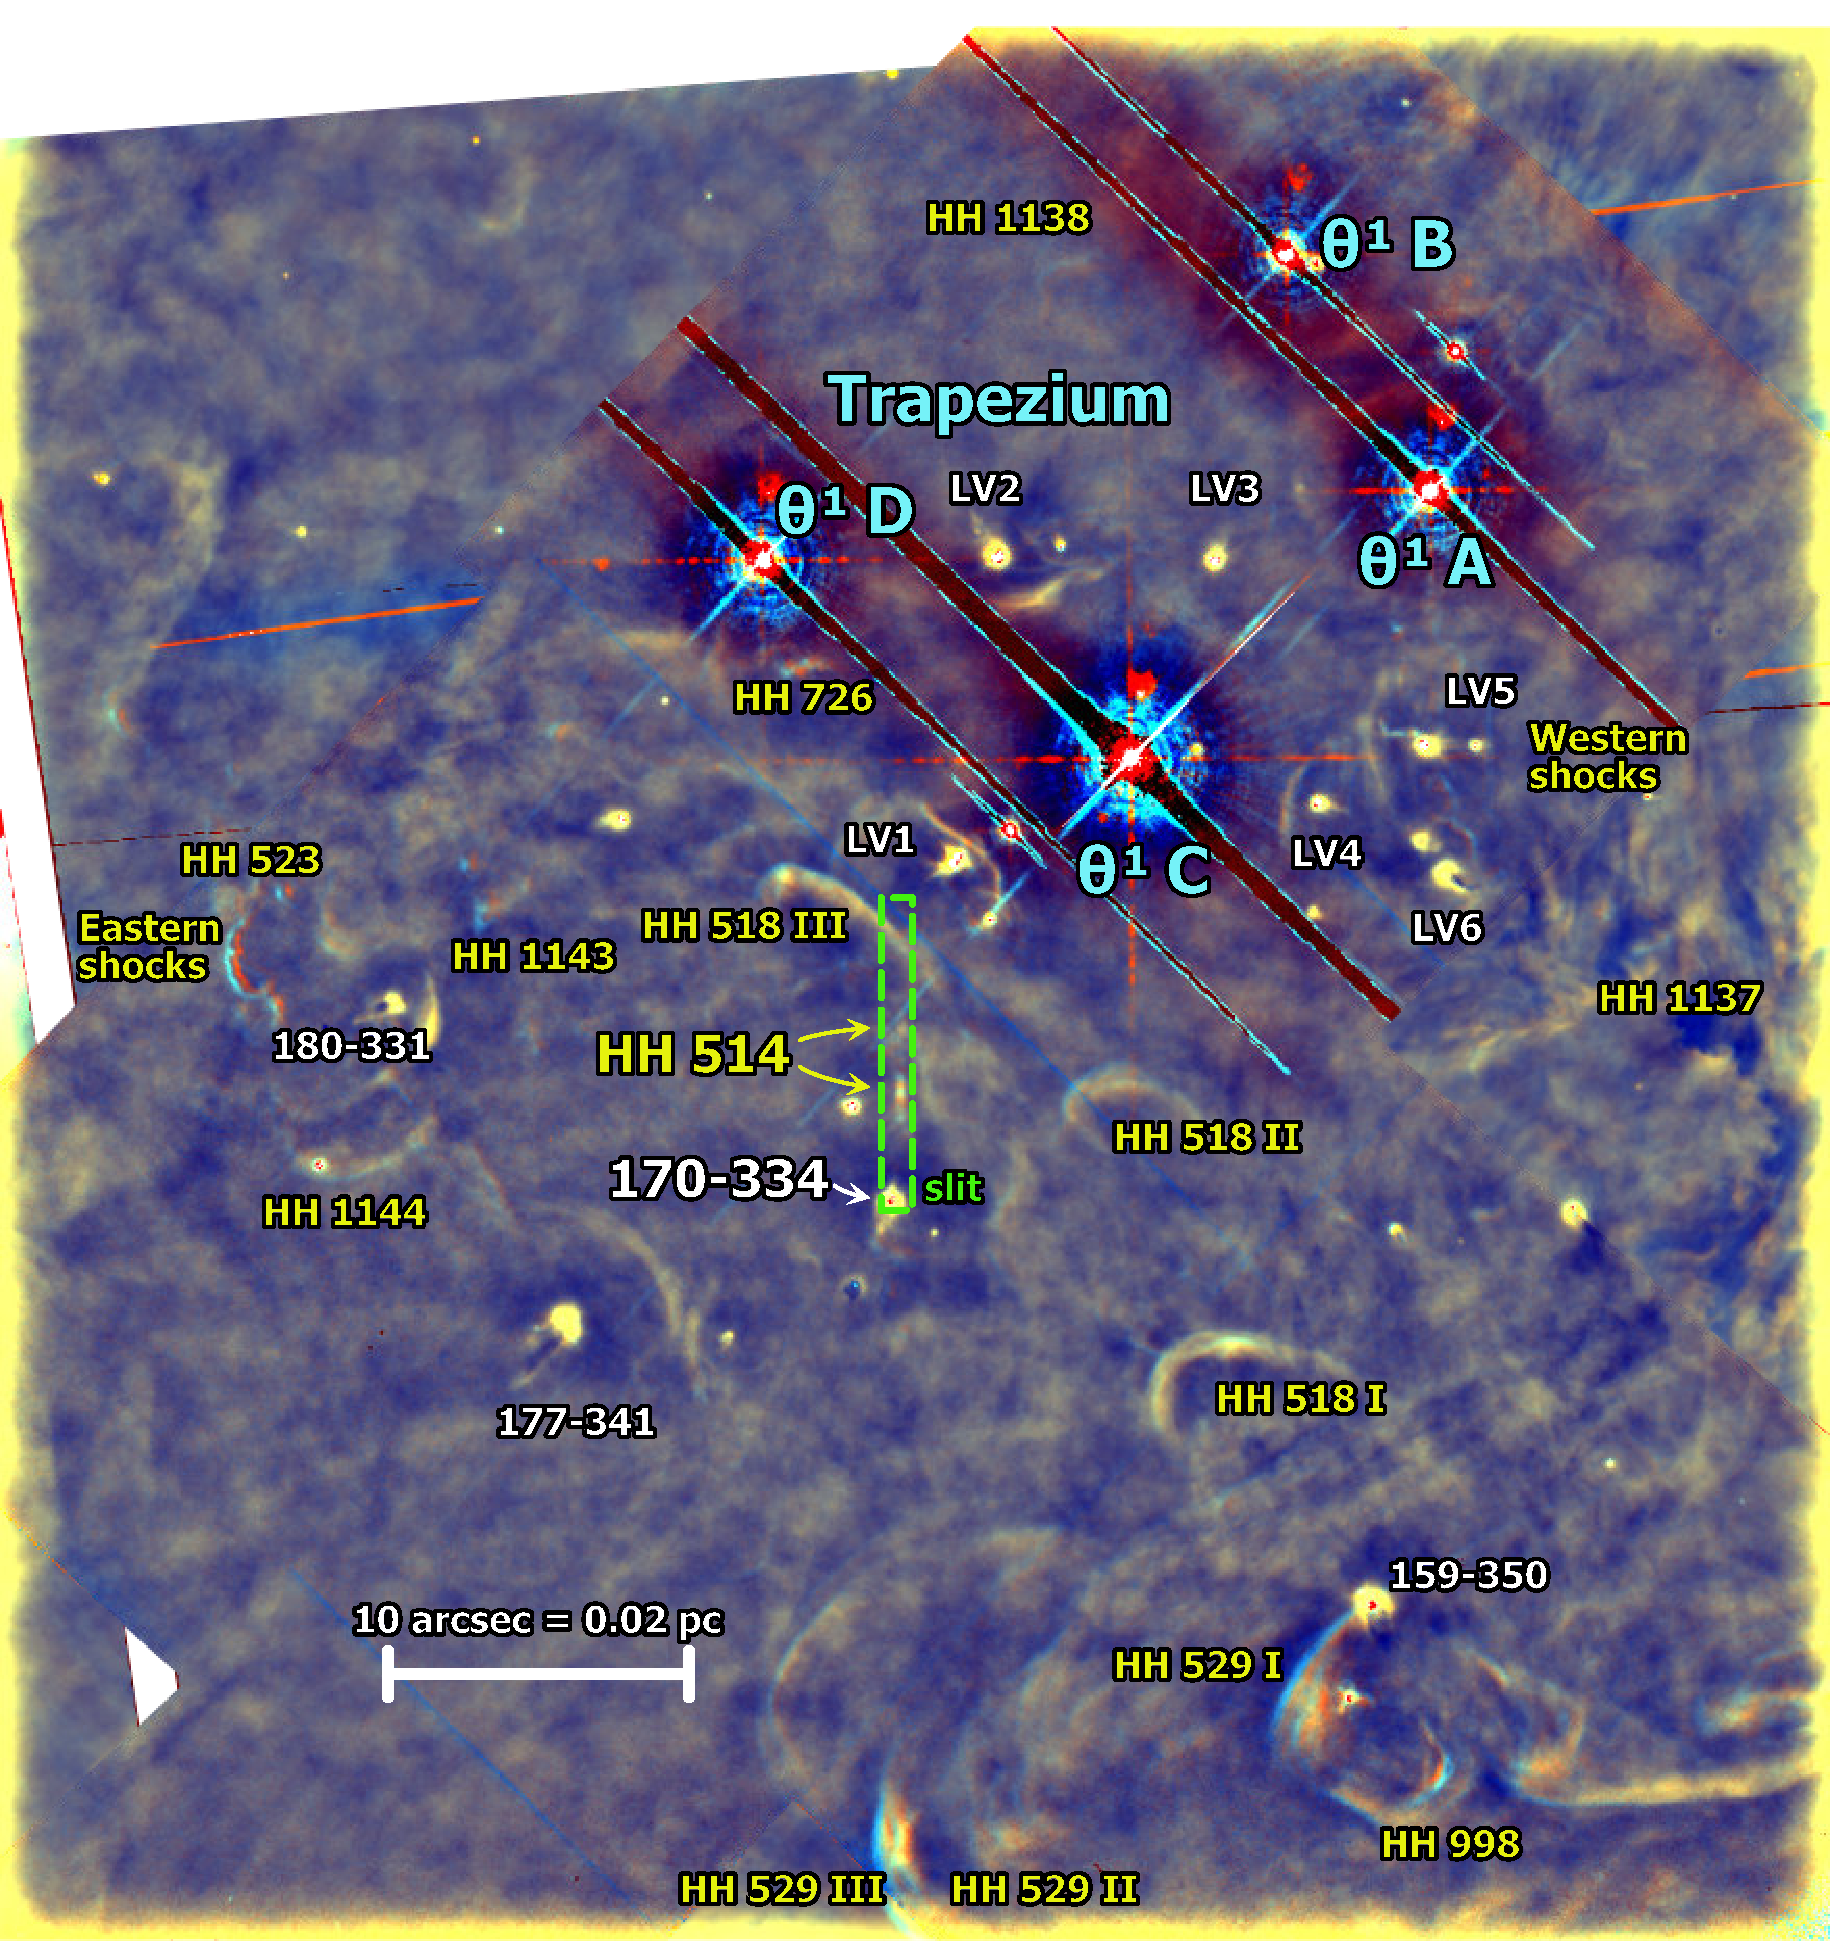
\includegraphics[width=\textwidth]{hh514-finding}
\caption{Aqui va imagen de HST}
\label{fig:hst}
\end{figure*} 



\section{Observations and data reduction}
\label{sec:data}

The observations were taken during the nights of 29 and 30 October, 2013, under clear conditions using UVES in the UT2 telescope of the VLT. The central coordinates of the 10 arcsec slit are: RA(J2000)=05$^h$35$^m$16$^s$.95, DEC(J2000)=$-$05$^{\circ}$23$'$33.72$''$ oriented along the north-south spatial axis as is shown in Fig.~\ref{fig:hst}. The slit aperture provides an effective spectral resolution of $\lambda/\Delta \lambda \approx 6.5 \text{ km s}^{-1}$ in the spectral range between 3100 and 10400 \AA. Analogously to the observations described in the articles on HH~529~II-III and HH~204 \citep[][hereinafter Paper~I and Paper~II, respectively]{mendez2021,mendez2021-2}, three exposures of 150s each of the star GD71 \citep{Moehler14a, Moehler14b} were taken during the same night under similar conditions to achieve the flux calibration of the science data. The configuration of the instrument and the data reduction procedure are described in detail in Paper~I while the main settings of the observations of HH~514 are shown in Table~\ref{tab:obs_set}. We define three spatial cuts along the observed slit as it is shown in Fig.~\ref{fig:cuts}, covering the main high-velocity components, separated about $\sim 150\text{ km s}^{-1}$ in the heliocentric velocity scale. We name the southernmost component (within Cut~1) as HH~514~I while the one located in the central cut as HH~514~II. The nebular emission of Cut~1 also contains the emission of the proplyd 170-337. The complete analysis of the physical conditions and chemical composition of this proplyd will be the subject of a future work (M\'endez-Delgado et al., in prep). In this work we will only mention some results on the abundance of S in 170-337 in Sec.~\ref{subsec:real_overabundance}, which is relevant for our analysis of HH~514~I-II. Panel (b) of Fig.~\ref{fig:cuts} shows several velocity components of lower velocity than HH~514, which emit mainly in lines of highly ionized ions such as [O\thinspace III] or [Ne\thinspace III]. Unfortunately, their emission is very weak in most spectral lines, so the determination of physical conditions and chemical abundances for those velocity components would not be reliable with the present data. In order to increase the contrast of the HH~514~I-II emission, which is rather weak compared to the main nebular background emission, we subtract Cut~3 --which contains only background nebular emission-- from Cut~1 and Cut~2, re-scaling its emission by the number of pixels of each cut. In addition to increasing the contrast of the HH~514~I-II emission, this subtraction procedure permits to remove sky and ghost contamination from the spectra of the HH object. We estimate the flux of the emission lines, their FWHM and their central wavelength by gaussian fittings using the SPLOT task of IRAF\footnote{IRAF is distributed by National Optical Astronomy Observatory, which is operated by Association of Universities for Research in Astronomy, under cooperative agreement with the National Science Foundation} \citep{Tody93} as is described in detail in Paper~I. We achieve the reddening correction by using the same procedure described in Paper~I and Paper~II \jorge{Creo que es de recibo mencionar que parametrización de la ley de extinción se usó (aunque sea la misma que en los papers I y II}. The resulting values of $\text{c}(\text{H}\beta)$, are presented in Table~\ref{tab:c_extin}. In Table~\ref{tab:sample_spectra} we include the relevant information for some of the emission lines of the spectrum of HH~514~I, as an example of the tables of the complete spectra that are provided as online material.

\begin{table}
\caption{Main parameters of UVES spectroscopic observations.}
\label{tab:obs_set}
%\begin{adjustbox}{width=\columnwidth}
\begin{tabular}{ccccc}
\hline
Date & $\Delta \lambda$& Exp. time  &Seeing &Airmass\\
 & (\AA) &  (s) & (arcsec)&\\
\hline
2013-10-30 & 3100-3885 & 5, 3$\times$180 &0.92&1.11\\
2013-10-30 & 3750-4995 & 5, 3$\times$600 & 0.87 & 1.15\\
2013-10-30 & 4785-6805 & 5, 3$\times$180 &0.92&1.11\\
2013-10-30 & 6700-10420 & 5, 3$\times$600 & 0.87 & 1.15\\
\hline
\end{tabular}
%\end{adjustbox}
\end{table}


\begin{figure*}
  \begin{minipage}{6cm}
    \centering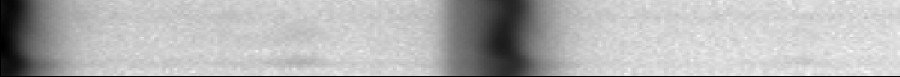
\includegraphics[height=2cm,width=\columnwidth]{2D_3729.pdf}
    \centerline{(a) [O\thinspace II] $\lambda 3729$.}
    \smallskip
  \end{minipage}
  \begin{minipage}{6cm}
    \centering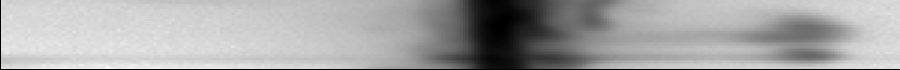
\includegraphics[height=2cm,width=\columnwidth]{2D_4959.pdf}
    \centerline{(b) [O\thinspace III] $\lambda 4959$.}
    \smallskip
  \end{minipage}
 
  \begin{minipage}{6cm}
    \centering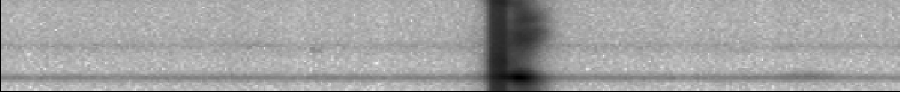
\includegraphics[height=2cm , width=\columnwidth]{2D_6300.pdf}
    \centerline{(c) [O\thinspace I] $\lambda 6300$.}
    \smallskip
  \end{minipage}
  \begin{minipage}{6cm}
    \centering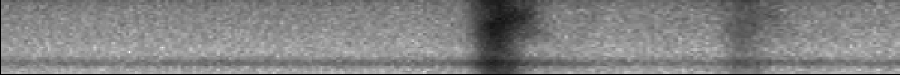
\includegraphics[height=2cm , width=\columnwidth]{2D_4649.pdf}
    \centerline{(d) O\thinspace II $\lambda 4649$.}
    \smallskip
  \end{minipage}
\begin{minipage}{12.0cm}
  \centering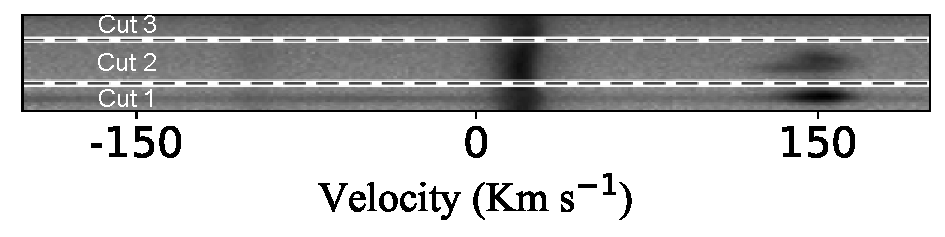
\includegraphics[height=4cm, width=\columnwidth]{2D_4658_cuts_named.pdf}
  \centerline{(e) [Fe\thinspace III] $\lambda 4658$.} 
\end{minipage}

\caption{\textit{Upper panels:} Sample of representative lines in the bi-dimensional spectrum. The Y axis corresponds to the spatial direction (up north, down south, see Fig.~\ref{fig:hst} for the spatial location of the slit) while the X axis is the spectral direction. All figures are centred at the rest-frame reference wavelength of each line. \textit{Bottom panel:} Emission of the [Fe\thinspace III] $\lambda 4658.17$ line as well as the limits and extension of the different spatial cuts extracted to analyse each velocity component. Cut 1 is at the bottom, which corresponds to the southernmost one. The spatial extension is 2.71 arcsec, 4.18 arcsec and 2.46 arcsec for cuts 1, 2 and 3, respectively. The velocity scale is heliocentric.}
\label{fig:cuts}
\end{figure*}




\begin{table}
\caption{Reddening coefficients for each component.}
\label{tab:c_extin}
%\begin{adjustbox}{width=\columnwidth}
\begin{tabular}{lccccc}
\hline
 & \multicolumn{2}{c}{$\text{c}(\text{H}\beta)$} \\
  & Nebular & High velocity\\
\hline
Cut 1 & - & $0.86 \pm  0.05$  \\
Cut 2 & $0.85 \pm 0.03$ &$0.75 \pm 0.07$\\
Cut 3 & $0.85 \pm 0.02$&-\\
\hline
\end{tabular}
%\end{adjustbox}
\end{table}





\section{Physical Conditions}
\label{sec:physical_cond}

We use the version 1.1.13 of PyNeb \citep{Luridiana15} and the atomic data set shown in Tables 9 and 10 from Paper~II to derive the physical conditions of the different gas  components analyzed in this work. The adopted electron density, $n_{\rm e}$, in the nebular components is a weighted average\footnote{The weights were defined as the inverse of the square of the error associated to each density diagnostic.} of the resulting values from the CEL diagnostics
[O\thinspace II] $\lambda3726/\lambda3729$, [S\thinspace II] $\lambda6731/\lambda6716$, [Cl\thinspace III] $\lambda5538/\lambda5518$, [Fe\thinspace II] $\lambda9268/\lambda9052$, [Fe\thinspace III] $\lambda4658/\lambda4702$ and [Ar\thinspace IV]  $\lambda4740/\lambda4711$.  We follow the maximum-likelihood procedure described in Sec.~4.2 of Paper~I to derive the physical conditions based on the [Fe\thinspace III] $\lambda \lambda $ 4658, 4702, 4734, 4881, 5011 and 5271 lines. As it was commented in Paper~I, with the adopted atomic data, [Fe\thinspace III] diagnostics are not adequately sensitive to density for values smaller than $10^{3} \text{ cm}^{-3}$, thus if a considerable part of the observed ionized gas has densities of the order or lower than that value (as it is expected in the nebular components), the resulting $n_{\rm e}$ may be biased to those of the densest zones along the line of sight. The value of $n_{\rm e}(\text{O\thinspace II})$ was derived with the available RLs of multiplet 1 and the results are highly consistent with the adopted average density.

In the plasma diagnostics of HH~514~I, there are two possible intersections of the temperature sensitive curve of [N\thinspace II] $\lambda5755/\lambda6584$ with the density sensitive ones, giving very different values of the electron temperature,  $T_{\rm e}$. One gives an extremely high density (larger than 10$^5$ cm$^{-3}$) (shown in Fig.~\ref{fig:plasma}) or an extremely high temperature (higher than 10$^{5}$ K at smaller densities than 10$^{4}$ cm$^{-3}$, not shown in Fig.~\ref{fig:plasma}). The [Fe\thinspace III] $\lambda4658/\lambda4702$, [S\thinspace II] $\lambda$4069/$\lambda$4076 and [O\thinspace II] $\lambda$7319+20/$\lambda$7330+31 density diagnostics confirm the first case. In HH~514~I-II we estimate the convergence of $n_{\rm e}-T_{\rm e}$ by using the [Fe\thinspace III] $\lambda \lambda$ 4658, 4702, 4734, 4881, 5011, 5271 CELs. The resulting density in  HH~514~I is $10^{5.37} \text{ cm}^{-3}$, one of the highest densities estimated in a photoionized nebula. 

In the case of HH~514~II, the convergence shows a higher dispersion in $n_{\rm e}-T_{\rm e}$ which seems to be due to the mixture of two or more gas components with similar velocities and notably different physical and/or ionization conditions. As it is shown in Fig.~\ref{fig:spatial_dis}, the spatial distribution along the slit of the intensity of the  [Fe\thinspace III] $\lambda 4658$ line centred at a heliocentric velocity of $\sim 150 \text{ km s}^{-1}$ is double-peaked in HH~514~II, which shows that at least two different gas components moving at a similar velocity are integrated in this part of the HH object. However, the separation into two spatial components results in a very low signal-to-noise spectra. Thus, the physical conditions and chemical abundances derived in HH~514~II are expected to be more uncertain than those in HH~514~I.

Based on the adopted density in each component, we estimate $T_{\rm e}$ through various diagnostics shown in Table~\ref{tab:pc}. In the nebular components, we define $T_{\rm e} \text{ (low)}$ as the weighted average of $T_{\rm e} (\text{[N\thinspace II]})$, $T_{\rm e} (\text{[O\thinspace II]})$ and $T_{\rm e} (\text{[S\thinspace II]})$ while $T_{\rm e} \text{ (high)}$ is the weighted average of $T_{\rm e} (\text{[O\thinspace III]})$, $T_{\rm e} (\text{[S\thinspace III]})$ and $T_{\rm e} (\text{[Ar\thinspace III]})$. It is noticeable that, despite of the extremely high density of HH~514~I-II, the temperature is consistent with the expected values in photoionization equilibrium. \cesar{No veo clara la discusión que he marcado en rojo. Es una diferencia muy pequeña, yo lo quitaría, incluida la nota el pie. Te parece? There it seems to be a slightly underprediction of , which would be expected to be equal to or greater than $T_{\rm e}(\text{[O\thinspace III]})$ due to temperature stratification} \footnote{\cesar{Photons with energies close to the photoionization threshold of the elements are more easily absorbed since the photoionization absorption cross section values decrease as the energy of the photon increases \citep{osterbrock06}. This causes the less energetic photons (with energies greater than the ionization threshold) to be absorbed first than the more energetic ones, which generally implies that the areas with a lower degree of ionization of the nebula are hotter. Since the ionization potential of S$^{2+}$ is lower than that of O$^{2+}$, we would expect, at first approximation, $T_{\rm e}(\text{[S\thinspace III]})\geq T_{\rm e}(\text{[O\thinspace III]})$.}}. \cesar{This behaviour of $T_{\rm e}(\text{[S\thinspace III]})$ may have a common origin with an apparent overabundance of S$^{2+}$ in HH~514~I-II. This is gonna be discussed in Sec.~\ref{sec:disc}.} \jorge{Estoy de acuerdo en quitarlo. A pesar de que en HH514-II parece significativo, no estamos del todo seguros y no aporta mucho} In both HH~514~I and HH~514~II, the estimation of $T_{\rm e} \text{ (low)}$ is quite uncertain, given the low critical density of the diagnoses available for this ionization zone and the high density of these objects. Due to this, and considering the similarity between $T_{\rm e}(\text{[O\thinspace III]})$ in both velocity components, we will adopt the $T_{\rm e} \text{ (low)}$ determined for  HH~514~I --the spectrum with the best signal to noise ratio-- as also representative for  HH~514~II.






\begin{table*}
\centering
\caption{Physical conditions determined from  several diagnostics.}
\label{tab:pc}
%\begin{adjustbox}{width=\textwidth}
\begin{tabular}{ccccc}
\hline 
 & \multicolumn{1}{c}{Cut 1} & \multicolumn{2}{c}{Cut 2} & \multicolumn{1}{c}{Cut 3} \\
Diagnostic & HH514-I & Nebula & HH514-II  & Nebula\\
\hline
& \multicolumn{4}{c}{$n_e$(cm$^{\text{-}3}$)}\\


[O\thinspace II] $\lambda$3726/$\lambda$3729 &  - &$5980^{+1160} _{-870}$&  - & $5610^{+960} _{-800}$\\

[O\thinspace II] $\lambda$7319+20/$\lambda$7330+31 &  263030: & - & - &- \\

[S\thinspace II] $\lambda$6731/$\lambda$6716 & - & $4150^{+1810} _{-1230}$&  -& $4240^{+1400} _{-1030}$\\

[S\thinspace II] $\lambda$4069/$\lambda$4076 & 218780: & - &-&-\\

[Cl\thinspace III] $\lambda$5538/$\lambda$5518 & - & $7640^{+970} _{-1020}$&  -& $7620^{+1070} _{-960}$\\

[Fe\thinspace II] $\lambda$9268/$\lambda$9052 & >75860 & $4500^{+9740} _{-3590}$ &  -& $3540^{+9190} _{-2760}$ \\

[Fe\thinspace III] $\lambda$4658/$\lambda$4702 & 234420: & $8490^{+2490} _{-2350}$& 57020: & $6430^{+2810} _{-2080}$\\

[Ar\thinspace IV]  $\lambda$4740/$\lambda$4711 & - &$6730^{+660} _{-690}$& - & $4800^{+570} _{-690}$\\


O\thinspace II$^{*}$  & - &$5640 \pm 510$&-&$4960 \pm 650$ \\

[Fe\thinspace III]$^{*}$ & $231820 \pm 12120$ & $8600 \pm 810$ & $74240 \pm 14220$& $7540\pm 1020$\\ 


\textbf{Adopted} &  \boldmath${231820 \pm 12120}$ &  \boldmath${6690 \pm 940}$&  \boldmath${74240 \pm 14220}$&  \boldmath${5490 \pm 1120 }$\\

 & \multicolumn{4}{c}{$T_e$ (K)}\\

T$\left(\mbox{He}\thinspace \mbox{I} \right)$ & $8710:$&$7790 ^{+570} _{-480}$ & $6010:$&$7570 ^{+490} _{-550}$\\

[N\thinspace II] $\lambda$5755/$\lambda$6584  & $12860^{+1240} _{-1170}$& $9750^{+230} _{-220}$&- &$9880^{+230} _{-250}$\\

[O\thinspace II] $\lambda \lambda$ 3726+29/$\lambda \lambda$7319+20+30+31 & $9180^{+1500} _{-630}$& $9500^{+740} _{-610}$& $7830^{+1430} _{-810}$&$10980^{+1040} _{-1320}$\\

[S\thinspace II] $\lambda \lambda$4069+76/$\lambda \lambda$ 6716+31& $20010^{+45030} _{-9150}$& $9410^{+950} _{-1220}$&-&$10090^{+2180} _{-1400}$\\

[O\thinspace III] $\lambda$4363/$\lambda \lambda$4959+5007& $8880^{+250} _{-210}$& $8490^{+90} _{-100}$ & $9330^{+260} _{-230}$& $8400^{+80} _{-70}$\\

[S\thinspace III] $\lambda$6312/$\lambda \lambda$9069+9531 & $8420^{+310} _{-400}$& $8630^{+330} _{-340}$& $8230^{+430} _{-560}$ & $8820^{+330} _{-310}$\\

[Ar\thinspace III]  $\lambda$5192/$\lambda$7136  & - & $8070^{+190} _{-160}$&-&$8320^{+230} _{-190}$\\

[Fe\thinspace III]$^{*}$ & $6840 \pm 1640$ & $8960 \pm 850$ & $8180 \pm 1410$& $7850 \pm 830$\\

\textbf{\boldmath${T_e}$ (low) Adopted} & \boldmath${11370 \pm 1820}$ & \boldmath${9530 \pm 100}$& \boldmath${11370 \pm 1820}$ & \boldmath${9920 \pm 200}$\\


\textbf{\boldmath${T_e}$ (high) Adopted} & \boldmath${8880 \pm 250}$ & \boldmath${8430 \pm 150}$ & \boldmath${9330 \pm 260}$ & \boldmath${8410 \pm 100}$\\

\hline
\end{tabular}
%\end{adjustbox}
\end{table*}

%RMS6742=9.787e-17
%upperlimit-1sigma=3.435577660528658e-17
%upperlimit-3sigma=1.0306732981585972e-16
%6742HB-1sigma=0.080953722395563323
%6742HB-3sigma=0.24286116718668996
%upper-lim-1sigma=6.99
%upper-lim-3sigma=7.47


\section{Ionic and Total Abundances}
\label{sec:ionic_total_abundances}

We derive ionic abundances of N$^{+}$, O$^{+}$, S$^{+}$, Cl$^{+}$, Ca$^{+}$, Fe$^{+}$ and Ni$^{+}$ based on CELs and using $T_{\rm e} \text{ (low)}$. We derive the abundances of Cl$^{2+}$ and S$^{2+}$ using $T_{\rm e} \text{ ([S\thinspace III])}$ and the ionic abundances of O$^{2+}$, Ne$^{2+}$, Cl$^{3+}$, Ar$^{2+}$, Ar$^{3+}$ and Fe$^{3+}$ using $T_{\rm e} \text{ (high)}$. \cesar{Eduardo, reescribe lo que he marcado en rojo, no lo veo claro ni en qué te basas para decirlo. In HH 514 I-II, we derive Fe$^{2+}$ and Ni$^{2+}$ using $T_{\rm e} \text{ (high)}$ while in the nebular component we use $T_{\rm e} \text{ (low)}$ since for the high velocity components, $T_{\rm e} \text{ ([Fe\thinspace III])}$ suggest a better association of Fe$^{2+}$ with the physical conditions of the gas of high degree of ionization}. In the case of Ca$^+$, we must take into account that its abundance may not be correct because the possible coexistence of Ca$^+$ outside the $^+$ \jorge{H$^+$ ionized?} volume, due to the low ionization potential of Ca. 

As discussed in Paper~II, some [Fe\thinspace II] and [Ni\thinspace II] lines can be produced mostly by continuum pumping instead of collisional excitation. We make sure that the estimation of the Fe$^+$ abundance is not affected by fluorescence by using lines of the lower  a$^4$F--a$^4$P levels  ($\lambda \lambda$ 7155, 8892, 9052, 9267) mostly populated by collisions \citep{Baldwin96}. In the case of Ni$^+$ the fluorescence effects may be larger, considering that the  levels involved in the transitions that give rise to the observed optical lines have the same multiplicity. However, if the density is high enough, collisional excitations may dominate the production of [Ni\thinspace II] lines. Following the same procedure described in equation 1 from Paper~II --based on the equation 8 from \citet{Bautista96}--, we estimate a critical density of $n_{\text{cf}}= 55860 \text{ cm}^{-3}$, from which collisions dominate over  fluorescence in the production of [Ni\thinspace II] $\lambda 7378$ line at the apparent distance of 12.61 arcsecs from $\theta^1$ Ori C. This implies that in HH~514~I and HH~514~II --regions with densities larger than $n_{\text{cf}}$--, we can directly calculate the abundance of Ni$^{+}$ based on the intensity of [Ni\thinspace II] $\lambda 7378$ line. However, this is not possible in the nebular components, where --due to the much lower density-- fluorescence should dominate.

In the spectrum of HH~514~I, we estimate an upper limit for the abundance of Fe$^{3+}$ based on the noise level of the continuum at $\sim 6743.30$\AA, where we would expect the emission of [Fe\thinspace IV] $\lambda6740$. We carefully estimated this upper limit, taking into account that at 6742.91\AA~ there may be a relatively weak telluric emission line \citep[][]{Hanuschik03}. However, since Cut~3 was subtracted from Cut~1, --rescaling to the same number of pixels-- to increase the contrast between the nebular emission and HH~514~I, any contamination by telluric lines has been eliminated. \jorge{Aquí es donde iría lo de las observaciones de OSIRIS.}

%na/nb=1/r**2_a/1/r**2_b= r**2_b/r**2_a= 12.61**2/63.98**2= 0.038845588175657815
%nb=55860

In the nebular spectra, we estimate the He$^{+}$, C$^{2+}$, O$^{+}$, O$^{2+}$ and Ne$^{2+}$ abundances making use of RLs following the same procedure described in Paper~I. In the case of HH~514~I and HH~514~II, we can  determine the abundances from RLs only for He$^{+}$. In this case, the adopted He$^{+}$ abundance is an average from the resulting values based on the available He\thinspace I singlet lines and triplet ones less affected by self-absorption effects (See Table D14 from Paper~I). The results are shown in Table~\ref{tab:ionic_abundances}. 

\begin{table*}
\centering
\caption{Ionic abundances derived in each kinematic component in logarithmic unit with $n(\text{H})=12$.}
\label{tab:ionic_abundances}
%\begin{adjustbox}{width=\textwidth}
\begin{tabular}{ccccccccccccc}
\hline
 & \multicolumn{1}{c}{Cut 1} & \multicolumn{2}{c}{Cut 2} & \multicolumn{1}{c}{Cut 3} & \\
Ion &  HH~514~I & Nebula & HH~514~II  & Nebula \\
\hline
 & \multicolumn{4}{c}{CELs}\\

N$^{+}$  & $6.88^{+0.28} _{-0.13}$ &$6.89 \pm 0.02 $  & $6.23^{+0.27} _{-0.14}$& $6.84 \pm 0.03 $\\

O$^{+}$ & $7.93^{+0.51} _{-0.18}$ & $7.81 \pm 0.03 $&$7.40^{+0.49} _{-0.19}$ & $7.69 \pm 0.05 $\\ 

O$^{2+}$ & $8.30^{+0.05} _{-0.04}$& $8.37 \pm 0.03$& $8.45^{+0.05} _{-0.04}$ &$8.38 \pm 0.02 $\\

Ne$^{2+}$ & $7.56^{+0.06} _{-0.05}$& $7.84^{+0.04} _{-0.03}$ & $7.79^{+0.06} _{-0.05}$&$7.82^{+0.03} _{-0.02}$\\

S$^{+}$ & $6.11^{+0.23} _{-0.12}$ & $5.50 \pm 0.04 $& $5.34^{+0.26} _{-0.14}$&$5.45 \pm 0.05 $\\

S$^{2+}$ & $7.39^{+0.07} _{-0.06}$ &$6.86^{+0.05} _{-0.04}$ & $7.35^{+0.09} _{-0.07}$&$6.84^{+0.05} _{-0.04}$\\

Cl$^{+}$ & - &$3.63 \pm 0.04 $&- &$3.60 \pm 0.04 $\\

Cl$^{2+}$ &- &$4.98^{+0.06} _{-0.05}$&- &$4.99^{+0.06} _{-0.05}$\\

Cl$^{3+}$ & - &$3.79 \pm 0.03 $&- &$3.92 \pm 0.03 $\\

Ar$^{2+}$ & $6.29 \pm 0.04 $& $6.31 \pm 0.03 $& $6.19 \pm 0.04 $&$6.31 \pm 0.02 $\\

Ar$^{3+}$ & - &$5.09^{+0.04} _{-0.03}$& -&$5.15^{+0.03} _{-0.02}$\\

Ca$^{+}$ & $3.71^{+0.20} _{-0.12}$ &- &-&-\\

Fe$^{+}$ & $6.14 \pm 0.05$ & $4.39 \pm 0.05$ & - &$4.32 \pm 0.02$\\ 

Fe$^{2+}$ & $7.14 \pm 0.02$ & $5.28 \pm 0.01$& $6.83 \pm 0.04$&$5.17 \pm 0.02$\\

Fe$^{3+}$ & < 6.99 &$5.62^{+0.10} _{-0.08}$& -&$5.78 \pm 0.12 $\\

Ni$^{+}$ & $4.94^{+0.15} _{-0.09}$ & - &-&-\\

Ni$^{2+}$ &$5.84^{+0.07} _{-0.06}$ & $4.32 \pm 0.03 $ &$5.62^{+0.08} _{-0.07}$&$4.25 \pm 0.04 $\\

 & \multicolumn{4}{c}{RLs}\\

He$^{+}$  &$10.95 \pm 0.04$  & $10.92 \pm 0.02$& $10.96 \pm 0.02$&$10.92 \pm 0.02$\\

C$^{2+}$  & -& $8.37 \pm 0.01 $ &-&  $8.37 \pm 0.01$ \\

O$^{+}$ & - & $8.17^{+0.04} _{-0.03}$& -& $8.19 \pm 0.05 $ \\

O$^{2+}$ & - & $8.61 \pm 0.05$ & - & $8.63 \pm 0.05$  \\

Ne$^{2+}$ & -&$8.04 \pm 0.06 $&-& $8.10 \pm 0.08 $ \\

\hline
\end{tabular}
%\end{adjustbox}
\end{table*}



%Fe3: se usan las lineas mas intensas de cada nivel superior de origen para promediar.


To estimate the total abundances of C, N, Ne, S and Ar, we use the Ionization Correction Factors (ICFs) from \citet{Amayo2021}. These ICFs, based on photoionization models of giant H~II regions, are consistent with the schemes shown in table~10 of Paper~I. However, they additionally provide the 1-$\sigma$ limits of their predictions, allowing the formal propagation of uncertainties associated to the ICF. In our nebular spectra, the calculation of the total abundances of O, Cl and Fe did not require ICF and were estimated from the sum of their ionic abundances. In the case of Ar, Ar$^+$ is estimated to contribute only 1 or 2 per cent of the total Ar abundance, having a negligible impact. We estimate the total abundance of Ni as $\text{Fe/Ni}=\text{Fe}^{2+}/\text{Ni}^{2+}$ based on their similar depletion and ionization patterns \citep[][]{mendez2021-2}. In the case of the He abundance in the nebular components, we use the ICF of \citet{kunthsargent83}. Since we have a reliable determination of the abundance of O$^+$ and O$^{2+}$ both with CELs and RLs, we derive the total abundances of He, Ne and C using the degree of ionization estimated from the ionic abundances determined from RLs. 


In the case of HH~514~I, we determine the total abundance of Fe as Fe/H = Fe$^{+}$/H$^{+}$+Fe$^{2+}$/H$^{+}$+Fe$^{3+}$/H$^{+}$, summing the estimated upper limit of 12+log(Fe$^{3+}$/H$^{+}$) = 6.99. At first approximation, the total abundance of Fe should be between $7.18 \pm 0.02$ and $7.40 \pm 0.02$, where the value of 12+log(Fe$^{3+}$/H$^{+}$) takes values between 0 and 6.99.  \citet{rodriguez05} provides two ICF(Fe) schemes, where the true Fe abundance should be between the limits predicted by both schemes, based on the observed O$^{+}$/O$^{2+}$ and Fe$^{2+}$/O$^{+}$ ratios. In our case, both ICFs match in the value of 7.50. Therefore, considering the observational uncertainties in the abundance of O$^{+}$, this suggest that the upper limit of the value of Fe$^{3+}$/H$^{+}$ should be close to its expected true value and therefore 12+log(Fe/H)$\approx 7.40 \pm 0.02$. 

It is remarkable that log(Ni$^{+}$/Fe$^{+}$) = $-1.20 \pm 0.16$, while log(Ni$^{2+}$/Fe$^{2+}$) = $-1.30 \pm 0.07$, which confirms the conclusions of \citet{mendez2021-2} about the similar ionization and depletion patterns of Ni and Fe. Furthermore, this demonstrate that the effects of fluorescence on our Ni$^{+}$ abundance determination are negligible, since the levels that give rise to [Ni\thinspace II] $\lambda 7378$ have the same multiplicity and thus the continuum pumping effects should be stronger than for [Fe\thinspace II] that depends on the metastability of the intermediate a$^4$F$_{9/2}$ level \jorge{Refrasearía un poco la frase anterior porque está algo confusa}. The estimated total abundances are shown in Table~\ref{tab:total_abundances}.


\begin{table*}
\centering
\caption{Total abundances. The units are logarithmic with $n(\text{H})=12$.}
\label{tab:total_abundances}
%\begin{adjustbox}{width=\textwidth}
\begin{tabular}{ccccccccccccc}
\hline
 & \multicolumn{1}{c}{Cut 1} & \multicolumn{2}{c}{Cut 2} & \multicolumn{1}{c}{Cut 3} & \\
Ion &  HH~514~I & Nebula & HH~514~II  & Nebula \\
\hline
 & \multicolumn{4}{c}{CELs}\\

N  & $7.43 ^{+0.59} _{-0.32}$ & $7.64 \pm 0.16$ &$7.36 ^{+0.58} _{-0.31}$ & $7.69 ^{+0.18} _{-0.16}$ \\ 

O  & $8.45 \pm 0.16$ & $8.48 \pm 0.02$ &$8.49 \pm 0.06$&$8.46 \pm 0.02$\\

Ne & $7.75 ^{+0.19} _{-0.15}$ & $7.97 ^{+0.11} _{-0.10}$& $7.84 ^{+0.11} _{-0.09}$ & $7.92 ^{+0.09} _{-0.08}$ \\ 

S  & $7.43 ^{+0.16} _{-0.12}$ & $6.92 ^{+0.07} _{-0.06}$& $7.49 ^{+0.17} _{-0.14}$ &$6.91 ^{+0.07} _{-0.06}$\\

Cl & - & $5.03 \pm 0.05$&- &$5.04 \pm 0.04$\\

Ar & $6.32 ^{+0.12} _{-0.10}$ & $6.34 ^{+0.06} _{-0.05}$ & $6.29 ^{+0.14} _{-0.12}$& $6.34 \pm 0.04$\\

Fe & $7.40 \pm 0.02$ & $5.80 \pm 0.07$ & - &$5.89 \pm 0.09$\\

%$^{b}$Fe & $7.50 ^{+0.07} _{-0.03}$ & $5.66 \pm 0.01$-$5.86 \pm 0.03$ &$7.35 ^{+0.10} _{-0.06}$-$7.79 ^{+0.27} _{-0.12}$ & \\

Ni & $6.10 \pm 0.08$ & $4.83 \pm 0.08 $&-&$4.96 \pm 0.10$\\

 & \multicolumn{4}{c}{RLs}\\

He  &$10.95 \pm 0.04$  & $10.95 \pm 0.02$ & $10.96 \pm 0.02$ & $10.95 \pm 0.02$\\

C & - &$8.45 ^{+0.07} _{-0.06}$&-&$8.45 ^{+0.07} _{-0.06}$\\ 

O  &  - & $8.74 \pm 0.04$ &-&$8.76 \pm 0.04$\\ 

Ne  & - &$8.17 ^{+0.13} _{-0.11}$&-&$8.26 ^{+0.18} _{-0.14}$\\

\hline
\end{tabular}
%\end{adjustbox}
%\begin{description}
%\item $^*$ Based on RLs. \\
%\item $^a$ Derived as Fe/H=Fe$^{+}$/H$^{+}$+Fe$^{2+}$/H$^{+}$+Fe$^{3+}$/H$^{+}$. In HH~514~I we sum the estimated upper limit of log(Fe$^{3+}$/H$^{+}$)+12=6.99. \\
%\item $^b$ Derived from the observed Fe$^{2+}$/O$^{+}$ ratio and the ICF schemes of \citet{rodriguez05}. The true Fe/H abundance should be within the limits demarcated by the ICFs.  \\
%\end{description}
\end{table*}


\section{Discussion}
\label{sec:disc}


\subsection{On the anomalous [S\thinspace III] emission in HH~514}
\label{subsec:under_TS3}

There are two results for HH~514~I and HH~514~II included in Tables \ref{tab:pc} and \ref{tab:total_abundances}  that we want to highlight: $T_{\rm e} \text{ ([S\thinspace III])}$ $<$ $T_{\rm e} \text{ ([O\thinspace III])}$ and that their S/H ratio is around 0.5 dex higher than the value found in the nebular gas. The abnormally large S abundance seems to rely mainly on the S$^{2+}$ one, which represents 91\% of the S/H ratio.

The observed trend of $T_{\rm e} \text{ ([S\thinspace III])}$ goes in the opposite direction to the usual temperature stratification observed in H~II regions and simple photoionization models fail to reproduce the observed result \citep[][]{Binette2012}. On the other hand, the overabundance of S is large enough to be produced by error in the assumed ICF (the abundance of S$^{2+}$ alone is higher than the total S abundance of the Orion Nebula). A first look could make us to suspect that neither $T_{\rm e} \text{ ([S\thinspace III])}$ nor the S$^{2+}$ abundance are real, but the product of errors in some part of our analysis of HH~514. In the following subsections we explore some scenarios that could explain the observed results.

\subsubsection{Errors in    atomic data for analyzing [S\thinspace III] lines?}
\label{subsec:atomic_data}

After analyzing different sets of transition probabilities and collision strengths of different ions, \citet{Juan-de-Dios17} conclude that the derived ionic abundances can have uncertainties of around 0.1-0.2 dex introduced by the atomic data when density is lower than $10^4$ cm$^{-3}$, but they can reach values up to 0.8 dex for higher densities. Since both HH~514~I and HH~514~II, have extremely high densities, we expect the uncertainties due to atomic data may be amplified in these objects. Given such expectations, we decided to explore the the effect of the atomic data on their  S$^{2+}$ abundance.

Instead of following the methodology of  \citet{Juan-de-Dios17} of analyzing all possible combinations of transition probabilities and collision strengths available in PyNeb. We will first focus our attention on transition probabilities, discarding those that give clearly wrong results. If we do not do this in the first place, we may include spurious values in the resulting abundance distribution, which would increase the uncertainties associated with the atomic data. Once this first step is done, we will check the available collision strengths, analyzing their impact on $T_{\rm e} \text{ ([S\thinspace III])}$ and the S$^{2+}$ abundance.

%\subsubsection{The transition probabilities }
%\label{subsubsec:As}

We use the observed intensity of [S\thinspace III] $\lambda \lambda 9531, 9069, 8829$ lines, arising from the common $^1$D$_2$ upper level and the [S\thinspace III] $\lambda \lambda 3722, 6312$ lines, emitted from the same $^1$S$_0$ level. Their intensity ratios depend exclusively on the transition probabilities. In Table~\ref{tab:atomic_data_test}, we compare the aforementioned [S\thinspace III] line intensity ratios observed in several positions and HH objects of the Orion Nebula and other Galactic {\hii} regions for which we have deep high-spectral resolution spectra with the line ratios predicted by the different atomic datasets.    

As it is well known, infrared [S\thinspace III] $\lambda \lambda 9531, 9069$ lines can be affected by telluric absorption bands \citep{Noll12}. In \citet{mendez2021} and \citet{mendez2021-2}, we mentioned that [S\thinspace III] $\lambda 9069$ was affected by telluric absorptions, while $\lambda 9531$ remained unaffected in the background emission of the Orion Nebula, while in the HHs both lines escaped to the absorption bands. Since in this work we are interested in analyzing the [S\thinspace III] $\lambda$9531/$\lambda$9069 line ratio, we correct the spectra from telluric absorptions around the aforementioned lines. We use the observations of the star GD71 from each data set, normalizing them with the standard tabulated flux. Then, the science spectra were divided by the resulting telluric transmission function around [S\thinspace III] $\lambda \lambda 9531, 9069$. The corrected intensities are shown in Table~\ref{tab:tellabs}. 

[S\thinspace III] $\lambda 3722$ is usually blended with H14. We can not simply subtract the emission of H14 using its theoretical line ratio with respect to other isolated observed H\thinspace I line, since it is well known that H\thinspace I emissions from high quantum numbers $n$ suffer deviations from case ``B'' \citep[][]{mesadelgado09, rodriguez20}. Even using  contiguous lines as H13 or H15 may introduce important deviations \citep[See Fig.~A2 of][]{rodriguez20}. Therefore, we consider that it is better to only consider the observations where the spectral resolution of the data allows the correct Gaussian deblending of the lines, where the resulting FWHM of [S\thinspace III] $\lambda 3722$ is consistent with that of the isolated [S\thinspace III] $\lambda 6312$ line.

The transition probabilities tested used are those available in version 1.1.13 of PyNeb and those from the CHIANTI data base V10 \citep[][]{Chianti10}, named by the following acronyms: LL93-HSC95-MZ82b-KS86 \citep[][]{LL93,HSC95,MZ82b, KS86}, MZ82b-HSC95-LL93\citep[][]{MZ82b,HSC95,LL93}, FFTI06 \citep[][]{FFTI06}, TZS19\citep[][]{TZS19} and CHIANTI \citep[][]{Tayal97,FFTI06, Hudson12}. These data encompass all those studied by \citet{Juan-de-Dios17}, in addition to include those from TZS19 and CHIANTI. In the case of the FFTI06 data file, it has been named as PKW09 in previous versions of PyNeb, alluding to \citet{Podobedova09}, who cited \citet{FFTI06}. 

As shown in Table~\ref{tab:atomic_data_test}, the LL93-HSC95-MZ82b-KS86 transition probabilities are notoriously inconsistent with the observed values in the $^1$D$_2$-$^3$P$_2$ transition (adopted from \citet{KS86}) that gives rise to the line $\lambda 9531$. This difference allows us to discard this data set. Respect to the other data sets, the most consistent ones with the observed line ratios are those of FFTI06 and those of CHIANTI. However, as shown in Fig.~\ref{fig:A_sii}, the differences between the remaining data sets are small in the most important transitions ($\lambda \lambda 3722, 6312, 8829, 9069, 9531$). In fact, if we take the average and the standard deviation of the 4 remaining sets, we obtain A$_{3722}=7.06 \times 10^{-01} \pm 5.26 \times 10^{-02}$, A$_{6312}=2.20 \pm 7.89 \times 10^{-02}$, A$_{8829}=6.42 \times 10^{-06} \pm 1.49 \times 10^{-06}$, A$_{9069}=2.00 \times 10^{-02} \pm 1.31 \times 10^{-03}$ and A$_{9531}=5.26 \times 10^{-02} \pm 3.45 \times 10^{-03}$. Of these, the one with the greatest deviation is A$_{8829}$, of around 23\%. However, this probability of transition has very little weight in the determination of $T_{\rm e} \text{ ([S\thinspace III])}$ and the abundance of S$^{2+}$ if a nebular line different than $\lambda 8829$ is used, which is always the case. Moreover, if we discard the dataset of TZS19, this deviation is reduced to 4\%. Once removed the LL93-HSC95-MZ82b-KS86 data set, the uncertainties associated with the transition probabilities seems to be of around $\sim 5$\% while the predictions are quite consistent with the line intensity ratios observed in Table~\ref{tab:atomic_data_test}. The previous results indicate that the transition probabilities tested are either jointly correct or jointly wrong. We will assume the first possibility. From now on, we adopt the transition probabilities of FFTI06, whose values have been used in Paper~I and Paper~II.

%\subsubsection{The collision strengths }
%\label{subsubsec:Omegas}
Analogously, we explore the sets of atomic collision strengths available in PyNeb: GMZ95 \citep[][]{GMZ95}, TG99 \citep[][]{TG99}, HRS12 \citep[HRS12][]{}, GRHK14 \citep[][]{GRHK14} and TZS19 \citep[][]{TZS19}. These data sets encompass all those analyzed by \citet{Juan-de-Dios17}, in addition to TZS19. The CHIANTI data base V10 adopted by default the collision strengths of HRS12, so we will not make a separate mention. After comparing the different data sets, as shown in Fig.~\ref{fig:omega_siii_zoom }, we obtain the following mean values with their associated dispersion at 10000K: $\Omega_{3722}=3.65\times 10^{-1}\pm3.14\times 10^{-2} $, $\Omega_{6312}=1.38 \pm4.27\times 10^{-2} $, $\Omega_{8829}=7.64 \times 10^{-1}\pm6.33\times 10^{-2} $, $\Omega_{9069}=2.28\pm1.96\times 10^{-1} $ and $\Omega_{9531}=4.00\pm2.56\times 10^{-1} $. The global dispersion is around $\sim 8$\% in almost all the analyzed lines, except for the auroral line [S\thinspace III] $\lambda 6312$, where the dispersion is smaller ($\sim 3$\%).

If we try to explain the low temperature of $T_{\rm e} \text{ ([S\thinspace III])}$ and the high abundance of S$^{2+}$ with errors in the collision strengths, the most direct way to modify this is by changing the  $\frac{\Omega_{\text{Auroral}}}{\Omega_{\text{Nebular}}}=\frac{\Omega(6312)+\Omega(3722)}{\Omega(9531)+\Omega(9069)+\Omega(8829)}$ ratio. When $\frac{\Omega_{\text{Auroral}}}{\Omega_{\text{Nebular}}}$ decreases, $T_{\rm e} \text{ ([S\thinspace III])}$ increases, with a fixed observed [S\thinspace III] $\frac{I(\lambda3722)+I(\lambda6312)}{I(\lambda 8829)+I(\lambda9069)+I(\lambda9531)}$ ratio. Increasing the value of the denominator is the most direct way if it is also desired to decrease the abundance of S$^{2+}$, which is usually determined from the intensity of the nebular lines $\lambda \lambda 9531, 9069$. However, modifications in $\Omega_{9531}, \Omega_{9069}, \Omega_{8829}$ within the dispersion values of $\sim8$\% are not enough to explain the anomalous results in $T_{\rm e} \text{ ([S\thinspace III])}$ and the abundance of S$^{2+}$.

So we will make an experiment. We will assume the the collision strengths are wrong, with $\Omega_{9531}, \Omega_{9069}, \Omega_{8829}$ being underestimated beyond the dispersion found. We will increase the values of $\Omega_{9531}, \Omega_{9069}, \Omega_{8829}$, until get $T_{\rm e} \text{ ([O\thinspace III])}=T_{\rm e} \text{ ([S\thinspace III])} $ in HH~514~I. This is a lower limit since it is likely that $T_{\rm e} \text{ ([S\thinspace III])} $ can be between $T_{\rm e} \text{ ([O\thinspace III])} $ and $T_{\rm e} \text{ ([N\thinspace II])} $ \citep[][]{Berg20}, the latter being generally hotter. To achieve this, the modifications needed are of the order of 40\%, 5 times larger than the dispersion found in the studied atomic data. In Table~\ref{tab:modified_data_omega} we show the $T_{\rm e} \text{ ([S\thinspace III])} $ and the S$^{2+}$ abundances derived in each object by adopting the transition probabilities of FFTI06, the derived $n_{\rm e}$ for each case and varying the collision strengths. In the last column of the table, we show the results obtained with the modified collision strengths of GRHK14, with $\Omega_{9531}, \Omega_{9069}, \Omega_{8829}$ increased by 40\%. 


Now we will analyze the repercussions of these modifications. Using these modified data, in HH~514~I and HH~514~II $T_{\rm e} \text{ ([S\thinspace III])}$ matches $T_{\rm e} \text{ ([O\thinspace III])}$ \footnote{Although this is natural for HH~514~I, since the atomic data were constructed to obtain $T_{\rm e} \text{ ([S\thinspace III])}= T_{\rm e} \text{ ([O\thinspace III])}$, the result for HH~514~II is independent.}, while the modification implies $T_{\rm e} \text{ ([S\thinspace III])}\approx T_{\rm e} \text{ ([N\thinspace II])}$ for the Orion Nebula. The latter would imply that the S$^{2+}$ and N$^{+}$ ions coexist almost exclusively in the zone of low degree of ionization. However, the large modifications that we carry out are not enough to obtain a \textit{normal}\footnote{Which should be consistent with the one obtained in the Orion Nebula.} abundance of S in the high-velocity components. If we adopt $\text{log(S/H)+12}=7.07 \pm 0.03$ from \citet{mendez2021-2} as reference, we still have an overestimation of 0.23 dex in the S abundance of HH~514~I. An analogous case occurs in HH~514~II. Moreover, this experiment would imply a $\text{log(S/O)}=-1.81 \pm 0.06$ for the nebular component, which is completely inconsistent with the solar values of $\text{log(S/O)}=-1.58 \pm 0.08$ \citep{lodders19}. Since both S and O are $\alpha$-elements, a constant abundance ratio is expected from their common nucleosynthesis. Therefore, following the logic \textit{Reductio ad absurdum}, we demonstrate that the assumed hypotheses are incorrect. Therefore, it is not possible that there are underestimates of the order of 40\% or more in the collision strenghts $\Omega_{9531}, \Omega_{9069}, \Omega_{8829}$. Since minor modifications to this factor are insufficient to obtain a temperature $T_{\rm e} \text{ ([S\thinspace III])} \geq T_{\rm e} \text{ ([O\thinspace III])}$ and an abundance of $\text{log(S/H)+12} \sim 7.07$ in HH~514, we conclude that possible errors in the atomic data are not by themselves the cause of the observed inconsistencies.

\subsubsection{Is the [S\thinspace III] emission affected by the shock?}
\label{subsec:shock_affected}

We discard that the low $T_{\rm e} \text{ ([S\thinspace III])}$ and the high abundance of S$^{2+}$ can be explained by effects of the shock between HH~514 and the surrounding gas. Once heated, the gas form a cooling zone emitting CELs out of photoionization equilibrium. The size of this cooling zone is inversely proportional to the density \citep[][]{Hartigan87}, and given the high density found in HH~514, we expect its effects to be negligible. Moreover, the emission from the cooling zone, if any, would affect $T_{\rm e} \text{ ([S\thinspace III])}$ in the opposite direction, increasing the observed [S\thinspace III] $I(\lambda 6312)/I(\lambda 9531)$ line intensity ratio. 

\subsubsection{Telluric absorption bands or sky emission?}
\label{subsec:tell_abs_sky_emmision}

At the observed wavelengths of [S\thinspace III] $\lambda \lambda 6312, 9069, 9531$ ($\lambda \lambda 6315.31,9073.60, 9535.87$), we do not find emissions arising from the sky or from the Orion Nebula that could be blended at our spectral resolution. In the case of telluric absorption bands: although we made a correction for telluric absorptions around $\lambda \lambda 9531, 9069$ in our spectra, the emission of HH~514 falls outside the absorption bands. In any case, the existence of absorption bands in [S\thinspace III] $\lambda \lambda 9531, 9069$ would fictitiously increase $T_{\rm e} \text{ ([S\thinspace III])}$ and decrease the S$^{2+}$ abundance, in the opposite direction to what is found.

\subsubsection{Errors in reddening correction?}
\label{subsec:errors_CHB}

The [S\thinspace III] $I(\lambda 6312)/I(\lambda 9531)$ line intensity ratio is highly dependent on reddening correction. However, if we suppose that $T_{\rm e} \text{ ([S\thinspace III])} \geq T_{\rm e} \text{ ([O\thinspace III])}$, then $\text{c}(\text{H}\beta)\geq 1.22$ which is at least 44\% higher than the estimated value based on the observed Balmer and Paschen H\thinspace I lines, an unlikely scenario.

\subsubsection{Have we overestimated the density?}
\label{subsec:ov_density}

Now lets suppose that we have overestimated the representative density of the [S\thinspace III] zone. This would imply that in HH~514~I, $T_{\rm e} \text{ ([S\thinspace III])} \approx 10200 \text{ K}$ if $n_{\rm e} \leq 10000 \text{ cm}^{-3}$ (See panel (a) from Fig.~\ref{fig:plasma}). However, even assuming this temperature, the abundance of S$^{2+}$ would be still overestimated. $T_{\rm e} \text{ ([S\thinspace III])} \approx 13000 \text{ K}$ would be necessary to fix the inconsistency, which is not achieved with any density value.

\subsubsection{Is the source of HH~514 sulphur-rich?}
\label{subsec:proplyd}

\citet{bally00} identified the origin of HH~514 in the proplyd 170-337. A plausible hypothesis could be that 170-337 is sulphur-rich and during the ejection of the material that gives rise to HH~514 the gas did not get well mixed. In our observations, 170-337 is within Cut~1. We interpolate the nebular emission above and beyond the spatial zone covered by 170-337, so that we can separate the proplyd emission from that of the Orion Nebula. When analyzing the spectrum of 170-337, we have obtained  $n_{\rm e}\approx 10^{5.85} \text{ cm}^{-3}$, while $T_{\rm e} \text{ ([O\thinspace III])} \approx T_{\rm e} \text{ ([S\thinspace III])}=8100 \text{ K}$. With the aforementioned physical conditions $\text{log(S/H)+12} \approx 7.08$ which is consistent with the value derived by \citet{mendez2021-2}. Therefore, the proplyd 170-337 does not show an overabundance of S. The complete analysis of 170-337 will be part of a following paper (M\'endez-Delgado et al. (in prep)). The intensity of the lines used to estimate the $n_{\rm e}$([S\thinspace II]) $\lambda$4069/$\lambda$4076, $T_{\rm e} \text{ ([O\thinspace III])} \lambda4363/\lambda5007$ and $T_{\rm e} (\text{ [S\thinspace III])} \lambda6312/\lambda9531$  and the ionic abundances of S ([S\thinspace II] $\lambda 4069$, [S\thinspace III] $\lambda 9531$ ) are presented in Table~\ref{tab:fluxes_proplyd}.


\subsubsection{The overabundance of S seems real}
\label{subsec:real_overabundance}

Since we have ruled out several scenarios that may produce an unrealistic overabundance of S (and a low $T_{\rm e} \text{ ([S\thinspace III])}$), it seems reasonable to affirm that the abundance of S in HH~514 is higher than in the Orion Nebula. However, the physical phenomenon that is causing this overabundance of S is not clear. It has to be related to the interaction of HH~514 and the surrounding environment, since we have seen that in the source of HH~514, the proplyd 170-337, the abundance of S is consistent with the rest of the Nebula. %Additionally, the S must have a special role in the phenomenon of interaction between HH~514 and the surrounding environment.

In planet-forming disks, the main sulphur reservoirs are not well known. Although the S is mostly in gaseous phase in the ISM, most of it is found in rocks in the solar system. The path from the ISM to the planet-forming disks is not well understood \citep[][]{Kama19}. Recently, \citet{Kama19} have suggested the existence of S in refractory dust or sulfide mineral reservoirs. These dust grains are relatively large. In a star-protoplanetary disk system, some of the material in the disk is accreted towards the star. However, the presence of an object, such as a planet immersed in the disk, can cause a pressure bump that can accumulate the largest dust particles \citep{Pinilla2012,Birnstiel16}, filtering them from the smaller dust grains and gas that can freely flow towards the star \citep[][]{Kama19}.

It is possible to recreate this scenario in the observed area of this work. As shown in Fig.~\ref{fig:hst}, in addition to 170-337, there are several proplyds and stellar objects surrounded by protoplanetary disks. If HH~514 pass through a protoplanetary disk where the S is accumulated in reservoirs of large dust grains, the shock could break them up, releasing the S into its gaseous phase. This process would increase the relative abundance of S/H, cooling down the gas through the emission of [S\thinspace III] CELs, reflected in a lower $T_{\rm e} \text{ ([S\thinspace III])}$. Since HH~514 propagates radially in the opposite direction to the observer, it is possible that this process only affects a relatively small area along the integrated line of sight, which would imply that the obtained overabundance of S is a lower limit to the real abundance in the zone where the dust reservoirs of S have been destroyed. This would also imply that the drop in temperature in this small zone would not be reflected in other ions, whose elements do not form dust grains or do so in more volatile compounds such as O, consistent with our determination of $T_{\rm e} \text{ ([O\thinspace III])}$ in HH~514.


\subsection{The total abundance of Fe and Ni}
\label{subsec:totalFeandNi}

In HH~514~I we are able to directly derive the abundances of Ni$^{+}$, Ni$^{2+}$, Fe$^{+}$ and Fe$^{2+}$. Despite of only having an upper limit to the abundance of Fe$^{3+}$, as mentioned in Sec.~\ref{sec:ionic_total_abundances}, the ICF schemes of \citet{rodriguez05} predict that the total abundance of Fe/H is equal to the sum of the abundances of Fe$^{+}$ and Fe$^{2+}$ and the upper limit of Fe$^{3+}$. New observations of HH~514~I with a longer exposure time to determine the line [Fe\thinspace IV] $\lambda 6739.80$ would allow us to obtain the total abundance of Fe without ICFs. Both the total abundances of Ni and Fe in HH~514~I are a factor 40 higher than the estimated values in the main emission from the Orion Nebula. Moreover, these values are consistent with the reference Solar values from \citet{lodders19}. This suggests that in HH~514~I all the dust grains with content of Fe and Ni could have been destroyed by the shock, releasing their content to the gaseous phase. This would allow, by the first time, to have a direct estimate of the total abundance of these elements without corrections for dust depletion. 
However, in connection with Sec.~\ref{subsec:real_overabundance}, if the scenario discussed is the one that is taking place and if the dust reservoirs of S are dominated by the FeS or NiS, then the derived abundances of Fe or Ni may not be representative of the gas of the Orion Nebula. However, if the S reservoirs are dominated by other sulfides, the abundances of Fe or Ni would remain unaltered, being representative of the Orion Nebula.

%This could be a milestone in the field, as the chemical composition of the Orion Nebula is representative of the Solar neighborhood. In addition, abundance of log(Fe/H)+12$\approx 7.40 \pm 0.02$ and log(Ni/H)+12$\approx 6.10 \pm 0.08$, are totally consistent with the Solar abundances \citep{lodders19}, which goes against the large variations in metallicity claimed by \citet{DeCia2021}. 

\subsection{On the kinematics of HH~514}
\label{subsec:kinematics}
Aqui podemos determinar con precision la velocidad tangencial de HH514. 

\section{Conclusions}
\label{sec:summary_and_conclusions}

Through high spectral resolution spectra from UVES at VLT and high spatial resolution imaging from the HST, we analyzed the physical conditions, chemical abundances and kinematics of the photoionized Herbig-Haro object HH~514 and the Orion Nebula. 
Due to the Doppler shift between the emission of the Orion Nebula and HH~514, we independently study the emission of two high-velocity components: HH~514~I and HH~514~II. These HHs are extremely dense: $n_{\rm e}(\text{HH~514~I})=10^{5.37} \text{ cm}^{-3}$ and $n_{\rm e}(\text{HH~514~II})=10^{4.87} \text{ cm}^{-3}$. However, they present temperatures consistent with those of photoionization equilibrium in the Orion Nebula, with $T_{\rm e} \text{ ([O\thinspace III])} \sim 9000\text{ K}$.

The total abundances derived from the high-velocity components are fully consistent with the abundances derived in the Orion Nebula with the exception of S, Fe, and Ni. In the case of S, the culprit of the overabundance is the S$^{2+}$ ion, which comprises 91\% of the total abundance. Furthermore, we found that $T_{\rm e} \text{ ([S\thinspace III])} < T_{\rm e} \text{ ([O\thinspace III])} $, which is difficult to explain under normal photoionization conditions \citep[][]{Binette2012}. We explore different possible explanations, as possible errors in the atomic data, observational errors or that the source of HH~514, the proplyd 170-337, can be rich in sulphur. After a detailed analysis we discard all the aforementioned scenarios. One possible hypothesis is the interaction of HH~514 with S reservoirs in a protoplanetary disk. The presence of a protoplanet or a large object in a protoplanetary disk can generate a pressure bump that filters the accretion of dust grains, favouring the accumulation of the largest grains, including sulfides. After its passage, the bowshock of HH~514 could destroy them, releasing their components to the gaseous phase.

In HH~514~I we directly obtain log(Fe/H)+12$=  7.40 \pm 0.02$ and log(Ni/H)+12$= 6.10 \pm 0.08$ without dust depletion correction models. These abundances are a factor 40 higher than those derived in the Orion Nebula and are highly consistent with the Solar abundance reference \citep[][]{lodders19}. This seems to indicate that all the dust grains containing Fe and Ni have been destroyed, releasing these elements to their gaseous phase. In this case, the derived Fe and Ni abundances of HH~514 would reveal directly the \textbf{true} content of these elements of the Orion Nebula. However, if the hypothesis we speculated to explain the overabundance of S takes place, and if in that case the largest reservoirs of S are compounds such as FeS or NiS, the derived abundances of Fe and Ni in HH~514~I might not be representative of the Orion Nebula and the consistency with solar values would be purely coincidental.





\section*{DATA AVAILABILITY}
The lines measured in the spectra are entirely available in online tables annexed to this article. Table~\ref{tab:sample_spectra} is an example of the content found in the online tables. The rest of information is found in tables or references of this paper.



\section*{Acknowledgements}

We acknowledge support from the Agencia Estatal de Investigaci\'on del Ministerio de Ciencia e Innovaci\'on (AEI-MCINN) under grant {\it Espectroscop\'ia de campo integral de regiones \ion{H}{2} locales. Modelos para el estudio de regiones \ion{H}{2} extragal\'acticas} with reference 10.13039/501100011033. JEM-D thanks the support of the Instituto de Astrof\'isica de Canarias under the Astrophysicist Resident Program and acknowledges support from the Mexican CONACyT (grant CVU 602402). JG-R acknowledges support from an Advanced Fellowship under the Severo Ochoa excellence program CEX2019-000920-S. The authors acknowledge support under grant P/308614 financed by funds transferred from the Spanish Ministry of Science, Innovation and Universities, charged to the General State Budgets and with funds transferred from the General Budgets of the Autonomous Community of the Canary Islands by the MCIU. 


%%%%%%%%%%%%%%%%%%%%%%%%%%%%%%%%%%%%%%%%%%%%%%%%%%

%%%%%%%%%%%%%%%%%%%% REFERENCES %%%%%%%%%%%%%%%%%%


\bibliographystyle{mnras}
\bibliography{Mendez}

\newpage
%%%%%%%%%%%%%%%%%%%%%%%%%%%%%%%%%%%%%%%%%%%%%%%%%%

%%%%%%%%%%%%%%%%% APPENDICES %%%%%%%%%%%%%%%%%%%%%

\appendix


\section{Some extra material}
\label{sec:apendix_A}

\begin{table*}
\caption{Sample of 15 lines of the HH~514~I spectrum. F$\left( \mbox{H}\beta \right)$=100. This is an example of the content found in the online tables for all spectra.}
\label{tab:sample_spectra}
%\begin{adjustbox}{width=\textwidth}
\begin{tabular}{ccccccccccccccccccccc}
\hline
$\lambda_0$ ( \AA ) & Ion & $\lambda_{\text{obs}}$( \AA ) & $v_r$ (Km s$^{-1}$) & FWHM (Km s$^{-1}$) & F$\left( \lambda \right)$/F$\left( \mbox{H}\beta \right)$ & I$\left( \lambda \right)$/I$\left( \mbox{H}\beta \right)$ & Err \% & Notes \\
\hline
4363.21 & $\mbox{[O}\thinspace \mbox{III]}$ & 4365.44 & 152.90 & 19.71 $\pm$ 1.43 & 2.103 & 2.478 & 6 &  \\
4471.47 & $\mbox{He}\thinspace \mbox{I}$ & 4473.78 & 155.02 & 22.45 $\pm$ 1.06 & 4.001 & 4.545 & 4 &  \\
4596.84 & $\mbox{[Ni}\thinspace \mbox{III]}$ & 4599.38 & 165.65 & 9.52 $\pm$ 5.51 & 0.241 & 0.262 & 38 &  \\
4607.12 & $\mbox{[Fe}\thinspace \mbox{III]}$ & 4609.42 & 149.71 & 19.77 $\pm$ 2.04 & 1.495 & 1.623 & 8 &  \\
4658.17 & $\mbox{[Fe}\thinspace \mbox{III]}$ & 4660.51 & 150.85 & 18.85 $\pm$ 0.07 & 16.852 & 17.983 & 2 &  \\
4667.11 & $\mbox{[Fe}\thinspace \mbox{III]}$ & 4669.40 & 147.38 & 24.46 $\pm$ 2.45 & 1.691 & 1.800 & 8 &  \\
4701.64 & $\mbox{[Fe}\thinspace \mbox{III]}$ & 4704.00 & 150.27 & 19.37 $\pm$ 0.36 & 8.265 & 8.693 & 3 &  \\
4734.00 & $\mbox{[Fe}\thinspace \mbox{III]}$ & 4736.33 & 147.47 & 21.52 $\pm$ 1.16 & 4.176 & 4.345 & 4 &  \\
4754.81 & $\mbox{[Fe}\thinspace \mbox{III]}$ & 4757.19 & 150.06 & 19.60 $\pm$ 0.99 & 3.388 & 3.499 & 4 &  \\
4769.53 & $\mbox{[Fe}\thinspace \mbox{III]}$ & 4771.92 & 150.28 & 20.36 $\pm$ 0.82 & 3.359 & 3.454 & 5 &  \\
4777.70 & $\mbox{[Fe}\thinspace \mbox{III]}$ & 4780.16 & 154.45 & 17.56 $\pm$ 1.69 & 2.062 & 2.118 & 7 &  \\
4814.54 & $\mbox{[Fe}\thinspace \mbox{II]}$ & 4817.00 & 153.41 & 17.43 $\pm$ 5.68 & 0.502 & 0.505 & 22 &  \\
4861.32 & $\mbox{H}\thinspace \mbox{I}$ & 4863.81 & 153.35 & 27.74 $\pm$ 0.27 & 100.000 & 100.000 & 2 &  \\
4881.07 & $\mbox{[Fe}\thinspace \mbox{III]}$ & 4883.58 & 154.04 & 18.42 $\pm$ 0.83 & 4.176 & 4.147 & 4 &  \\
4930.64 & $\mbox{[Fe}\thinspace \mbox{III]}$ & 4933.18 & 154.50 & 20.84 $\pm$ 3.43 & 1.565 & 1.527 & 12 &  blend with [O\thinspace III] 4931.23 \\
\hline
\end{tabular}
%\end{adjustbox}
\end{table*}






\begin{figure*}
  \begin{minipage}{7.5cm}
    \centering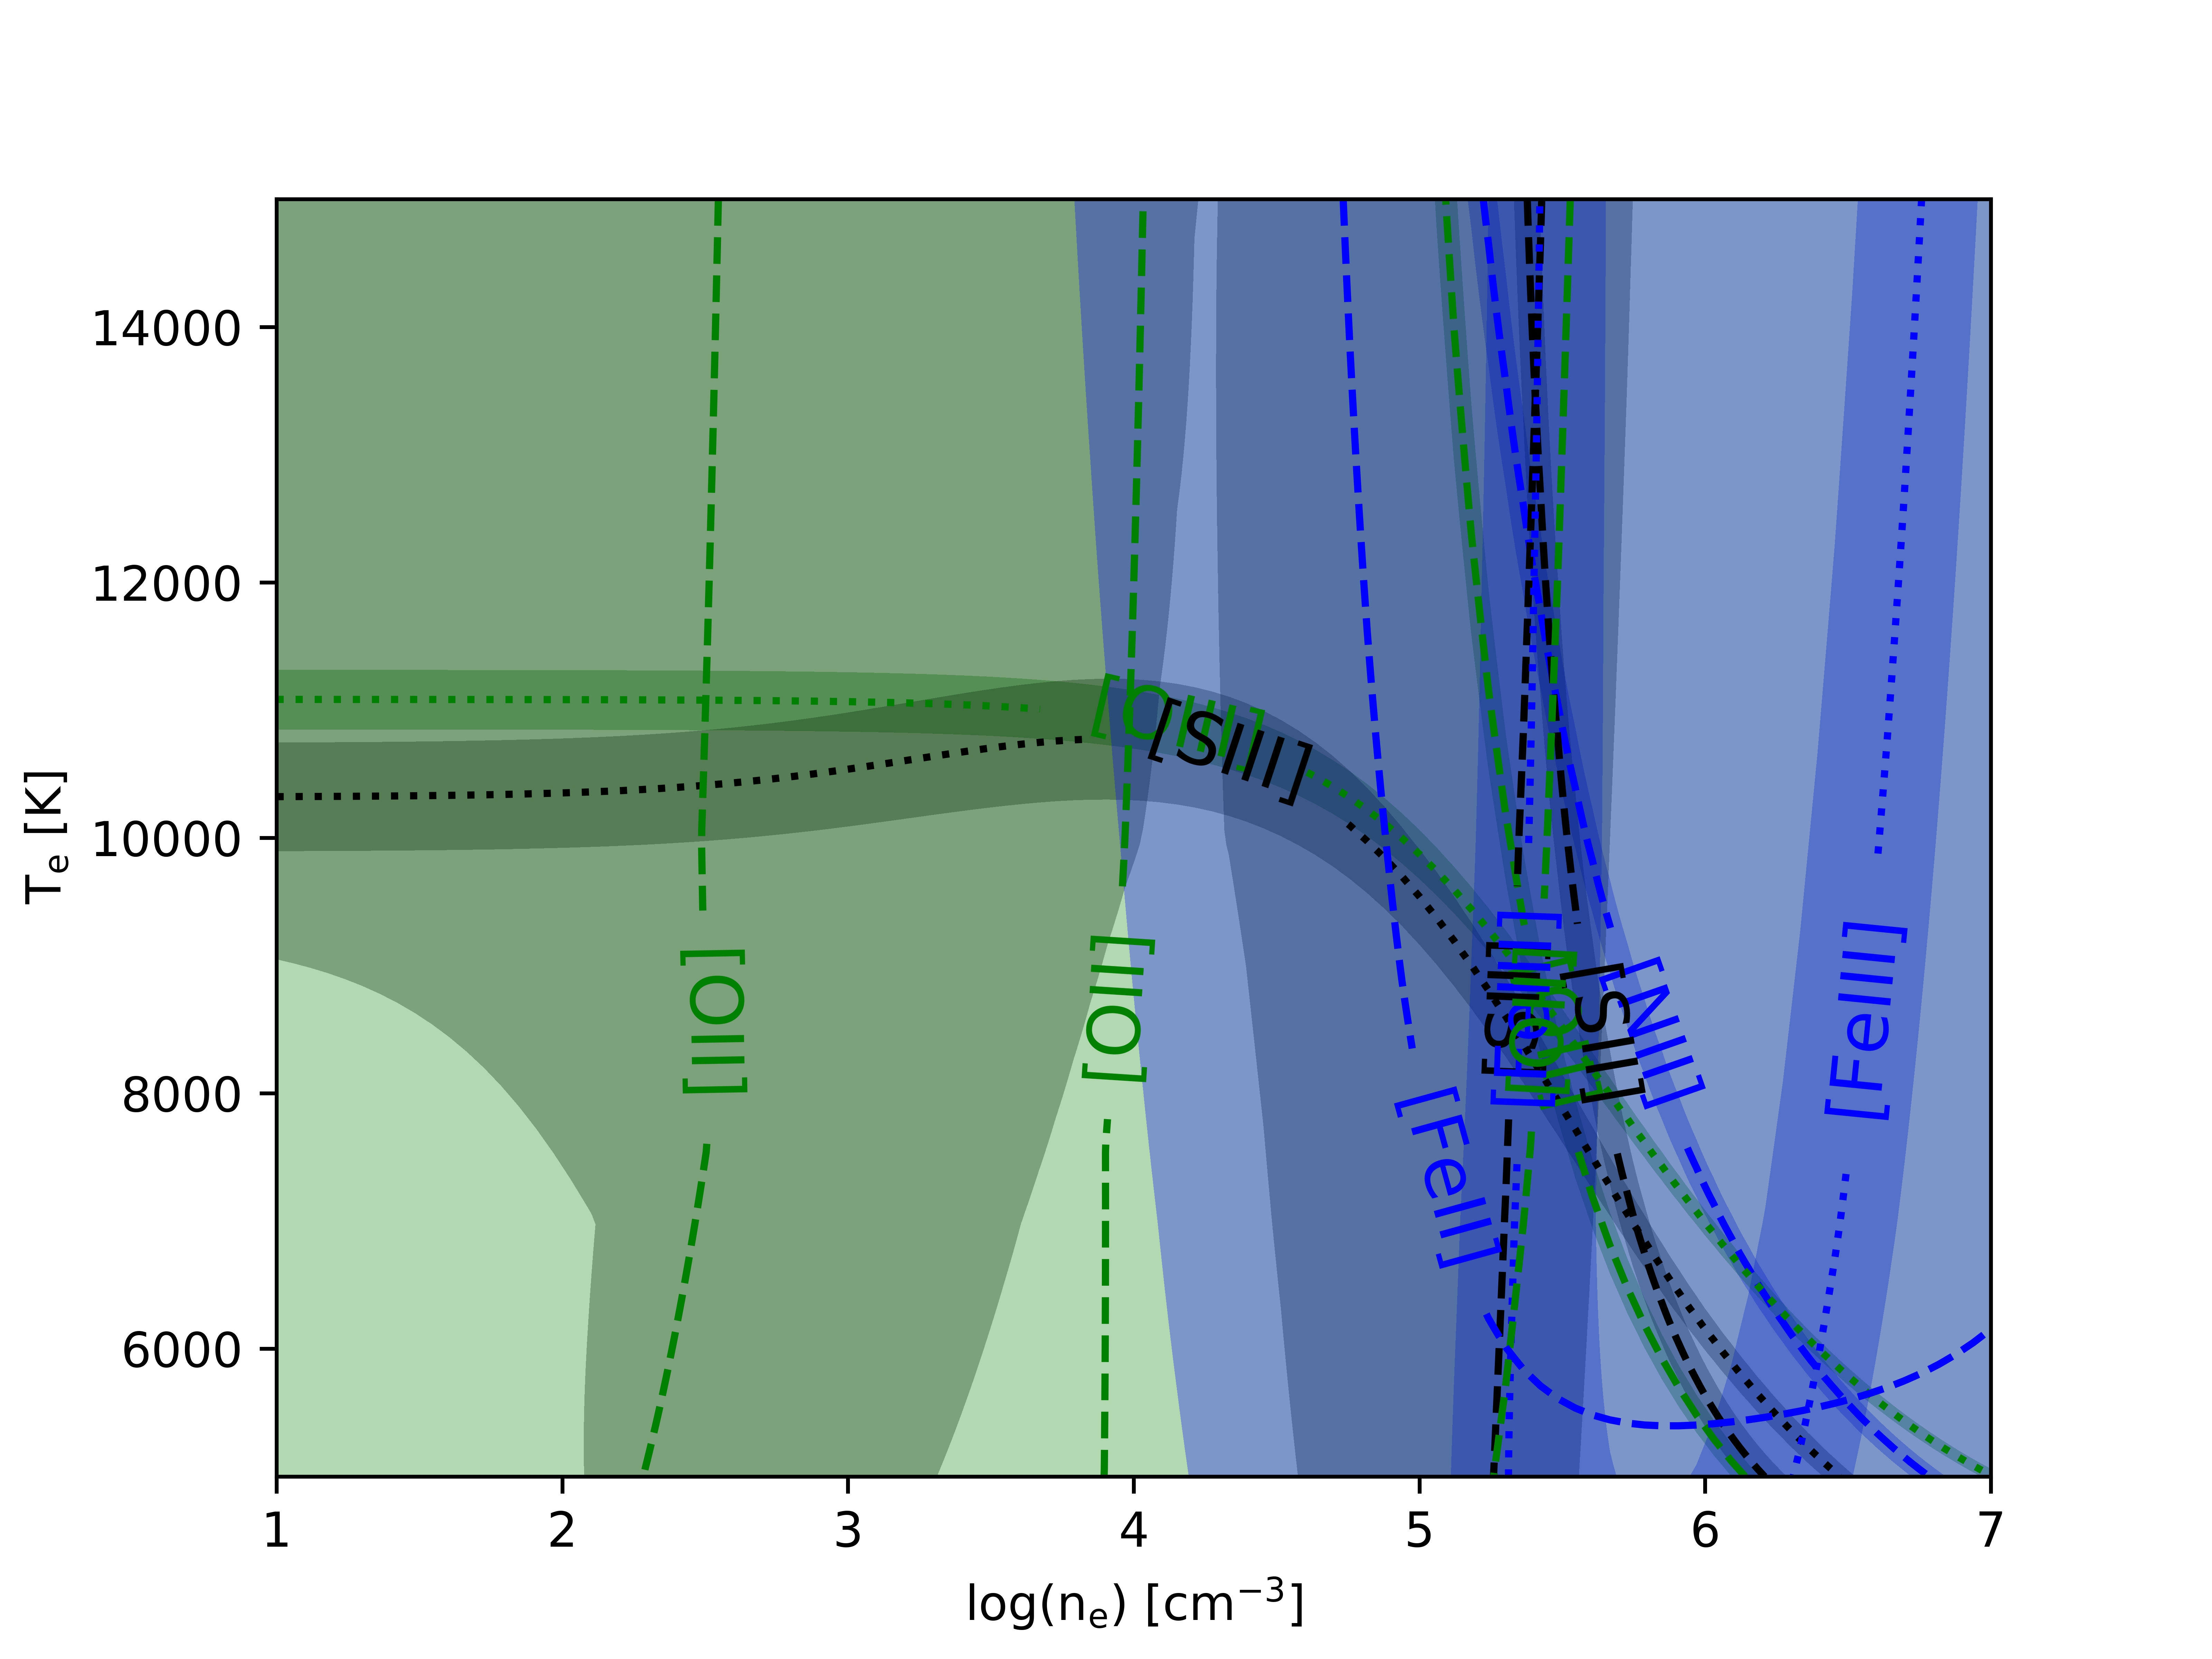
\includegraphics[height=4cm,width=\columnwidth]{HH514I.png}
    \centerline{(a) Cut~1, HH~514~I.}
  \end{minipage}
  \begin{minipage}{7.5cm}
     \centering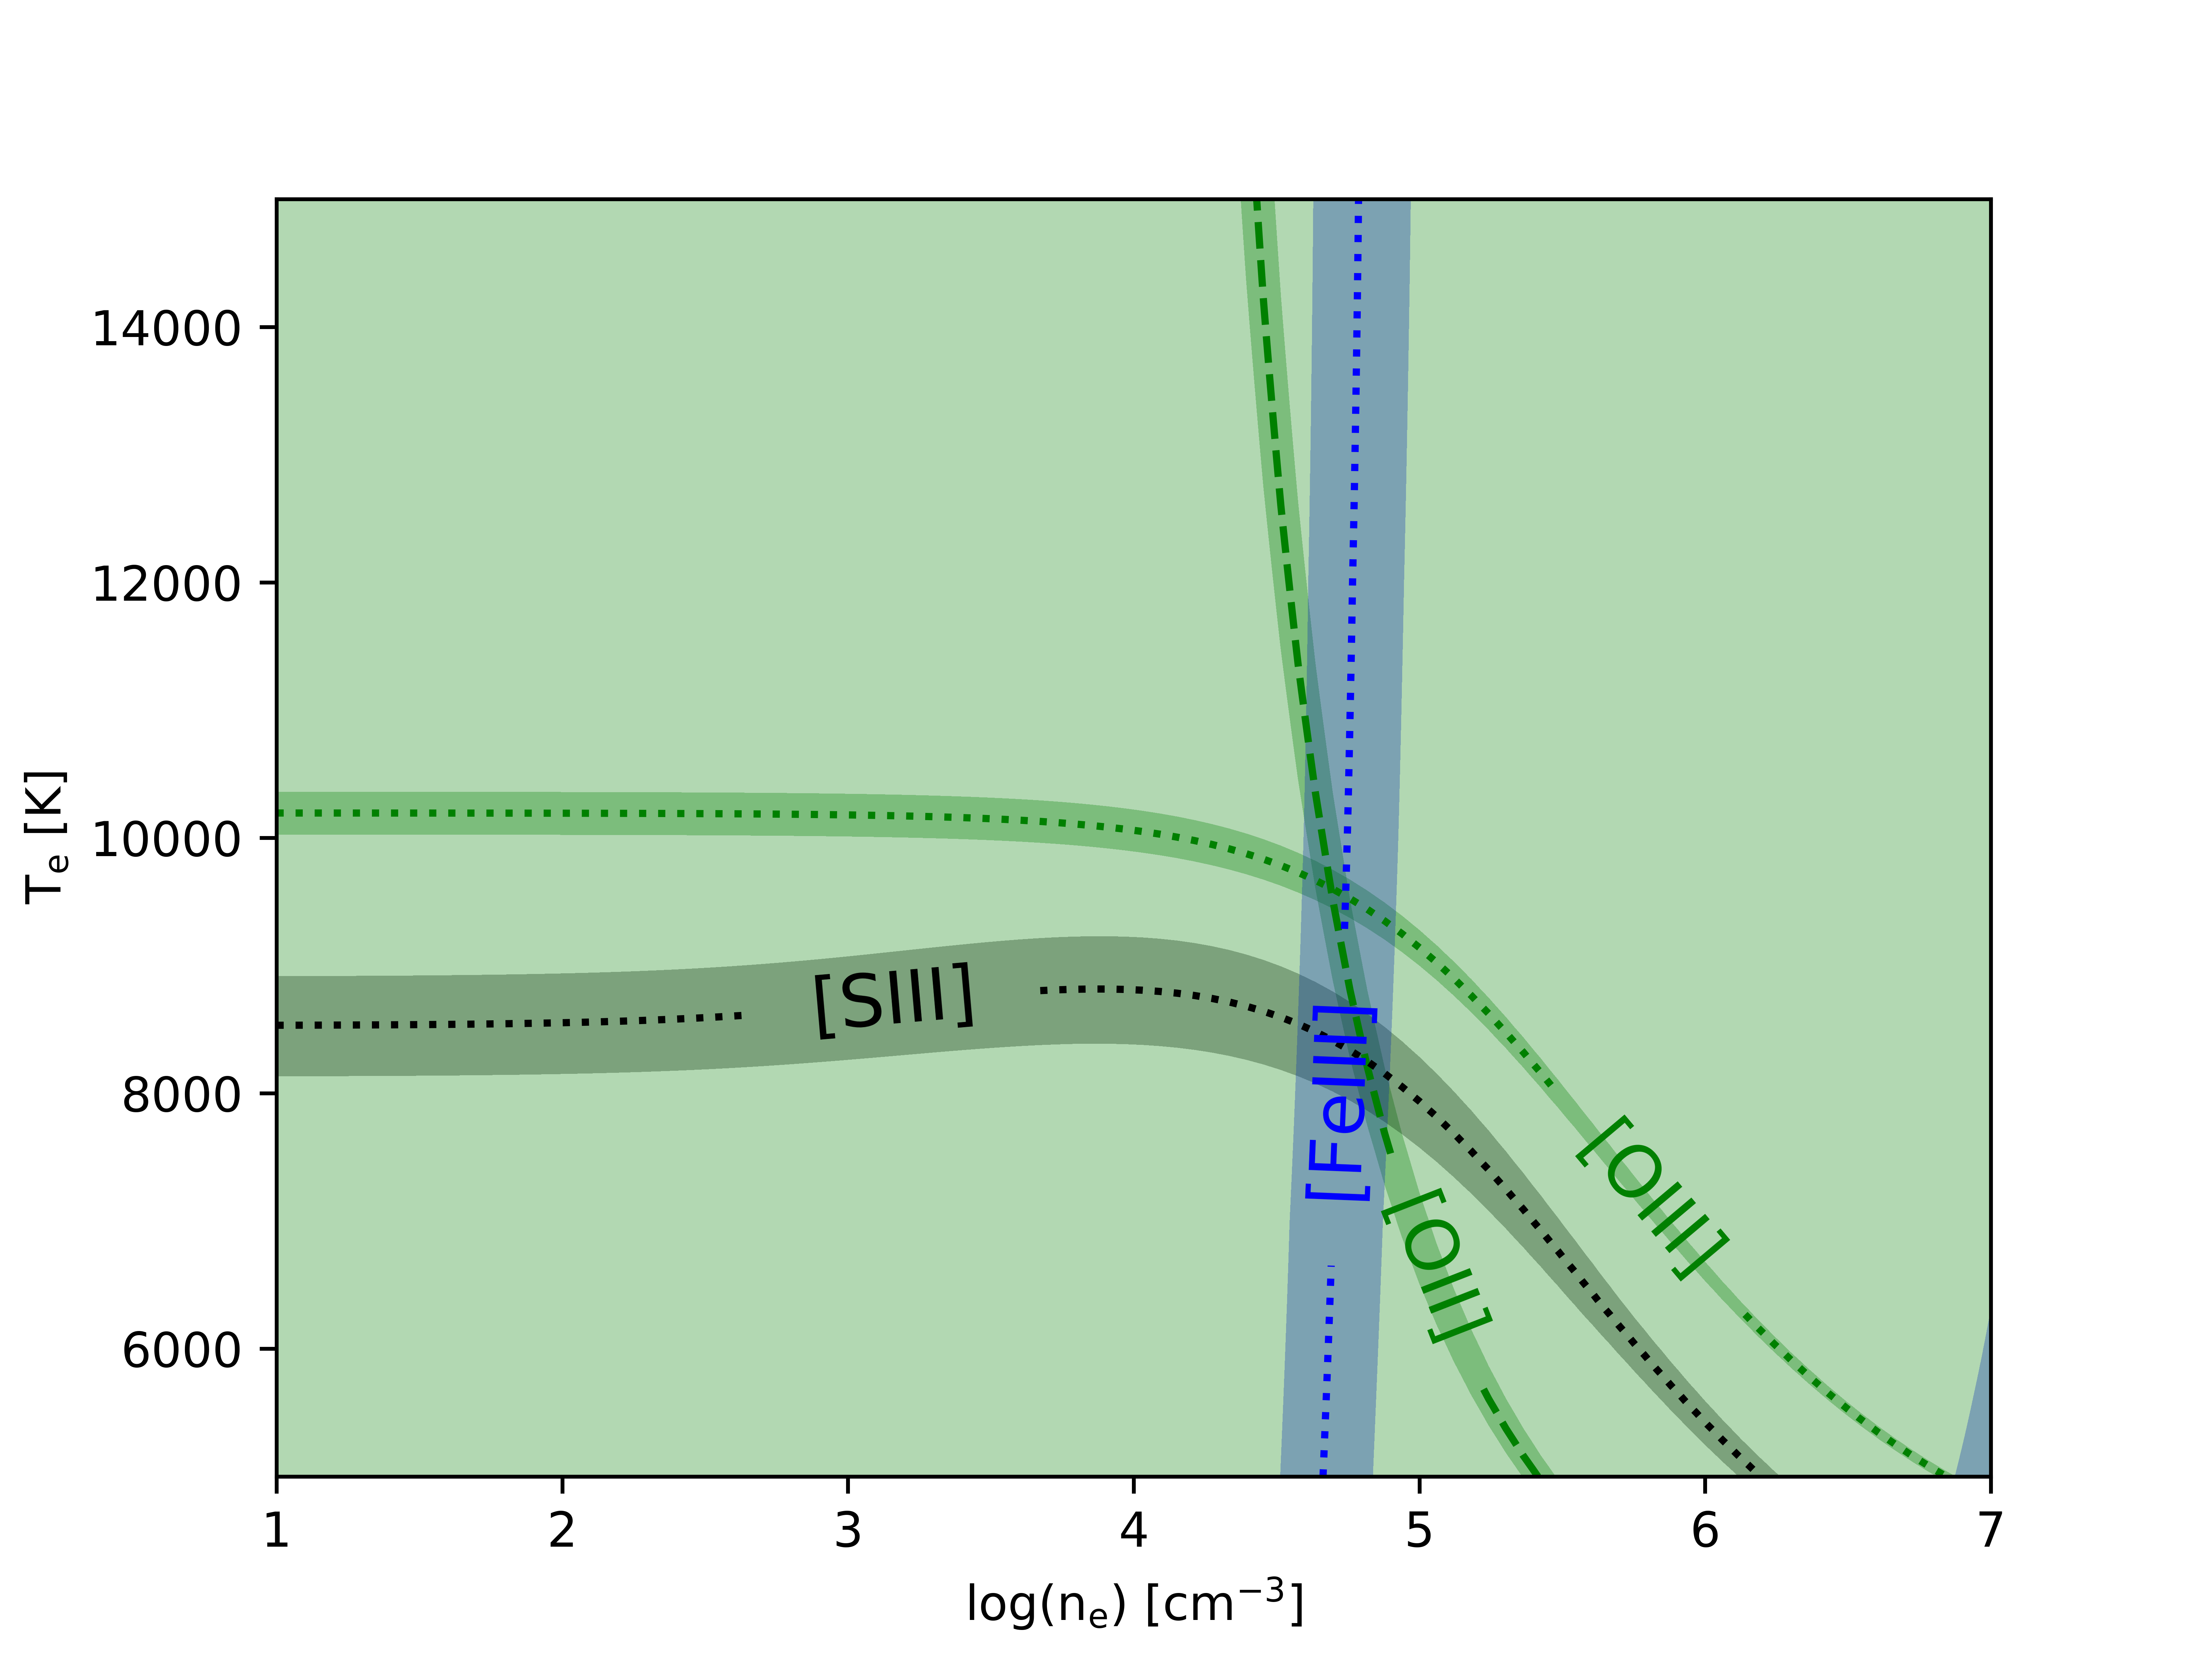
\includegraphics[height=4cm,width=\columnwidth]{HH514II.png}
    \centerline{(b) Cut~2, HH~514~II.}
  \end{minipage}
 
  \begin{minipage}{7.5cm}
   \centering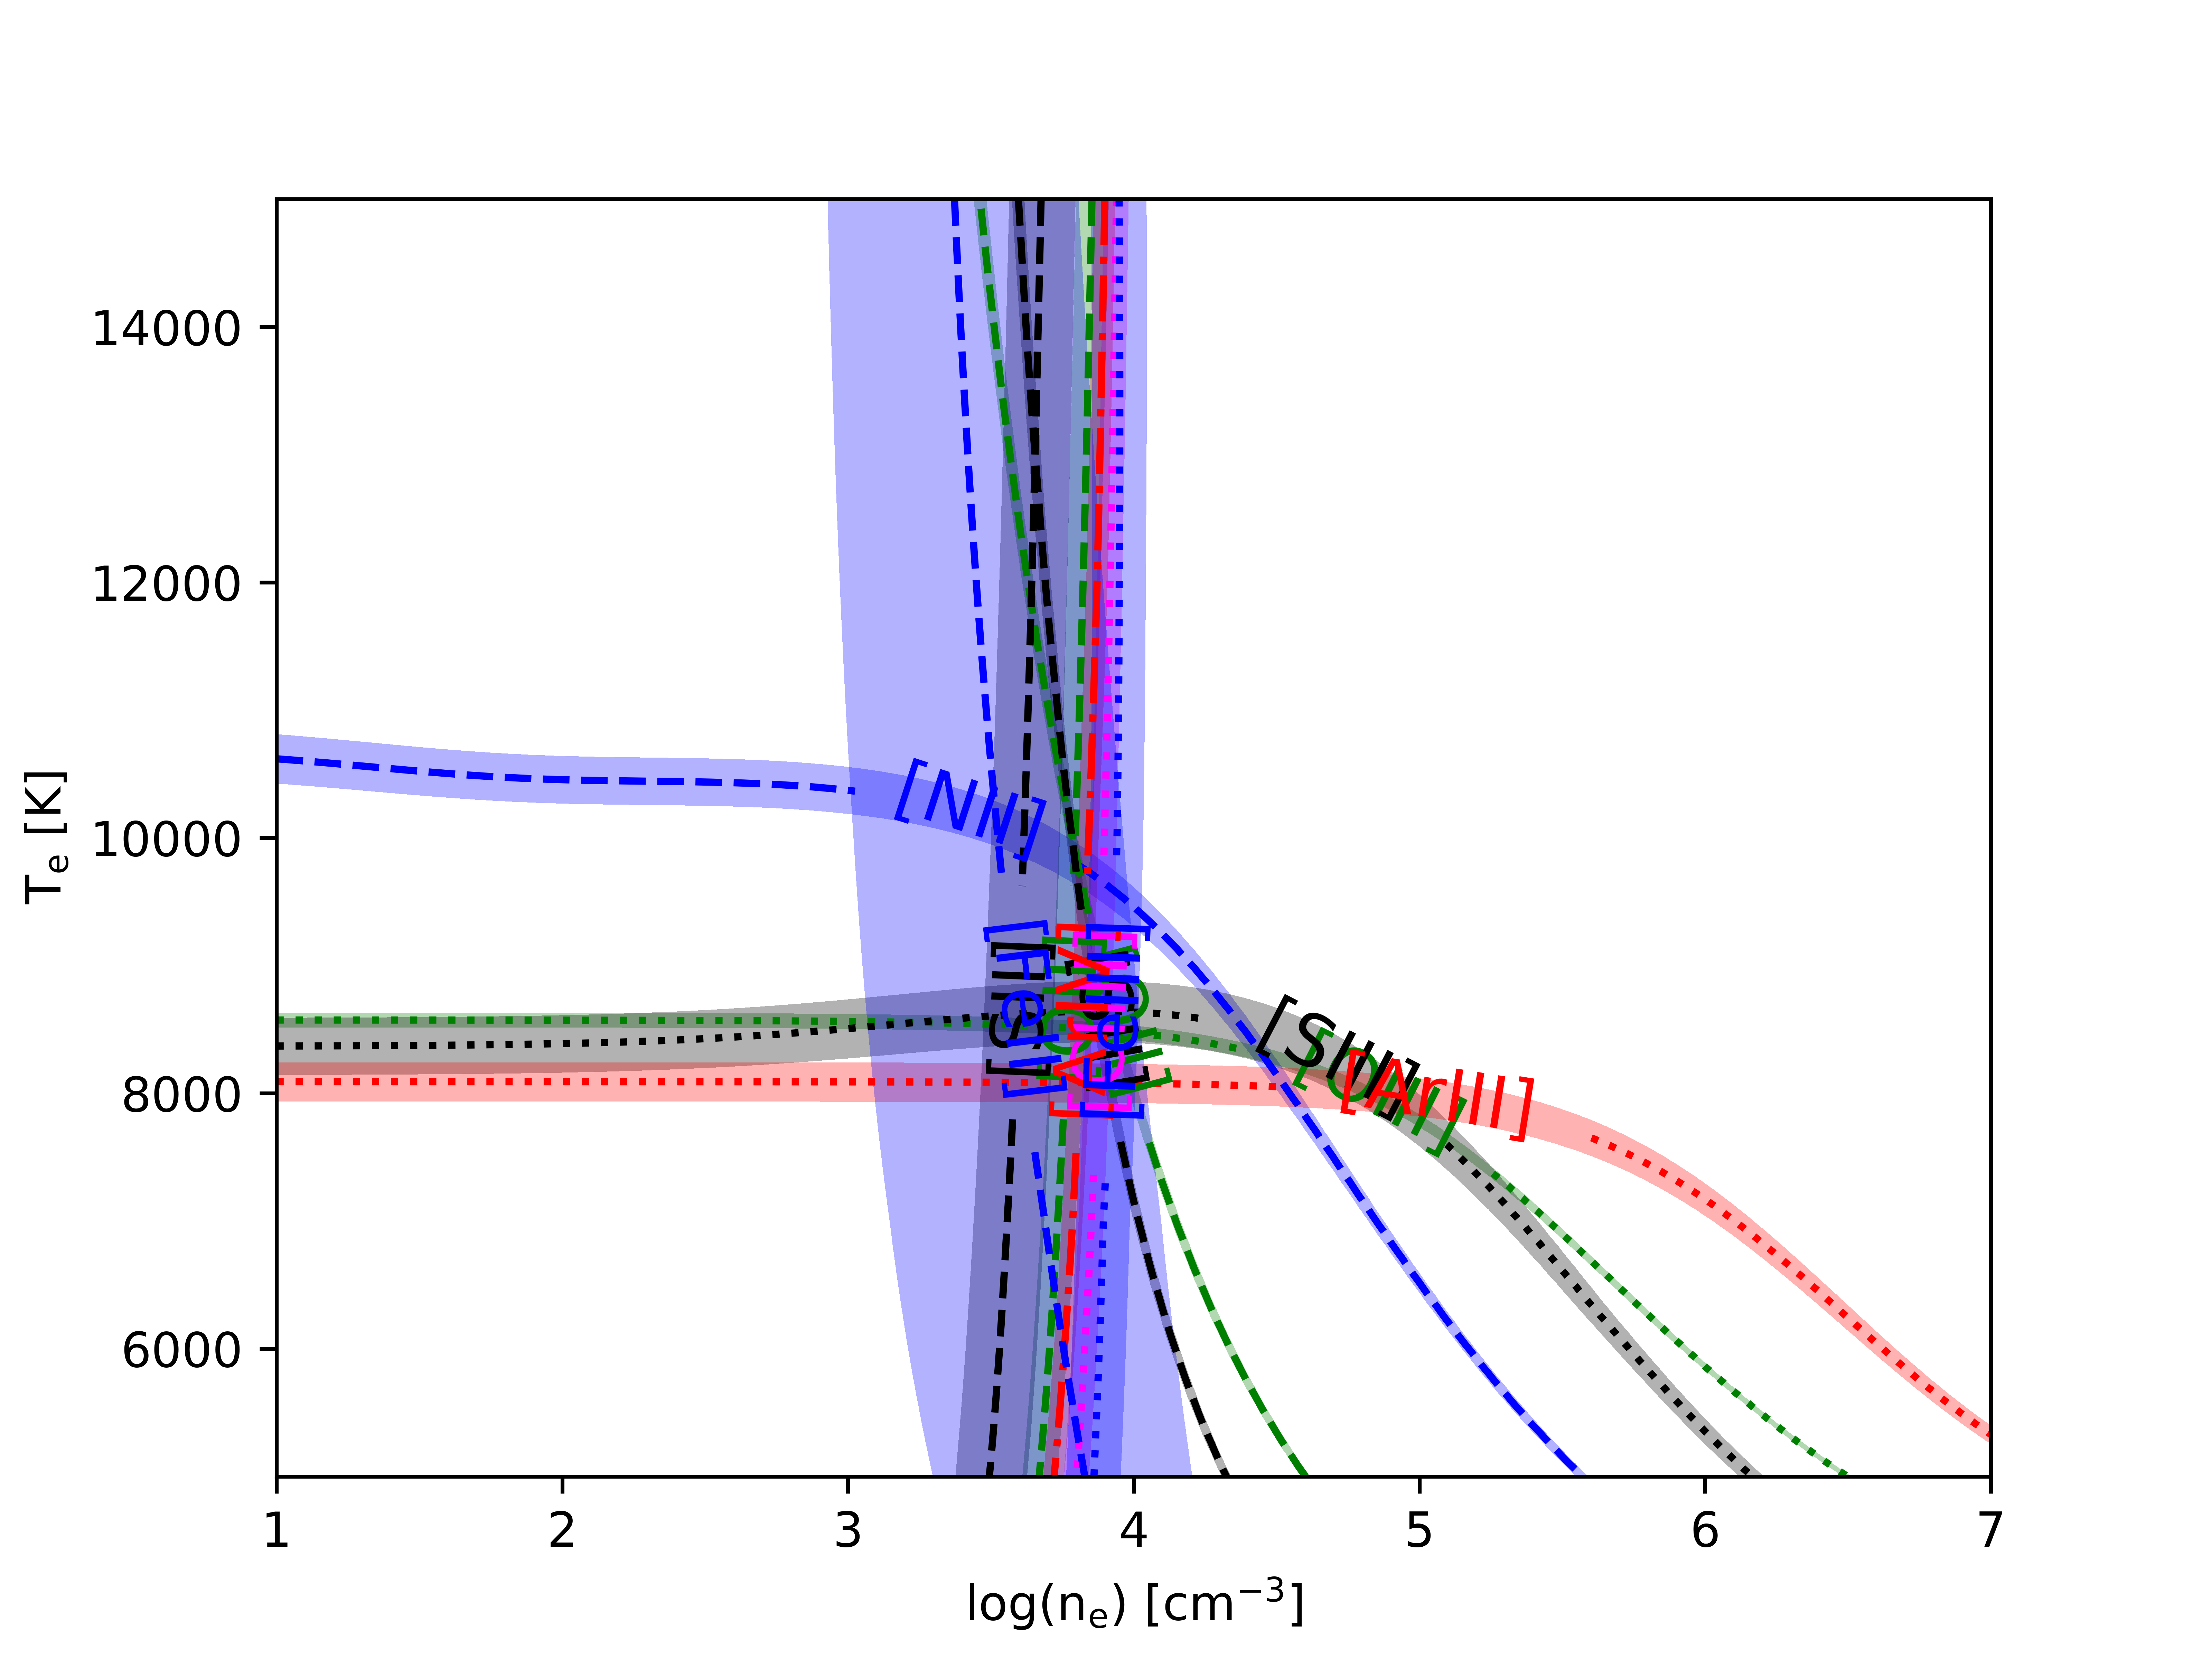
\includegraphics[height=4cm,width=\columnwidth]{neb_cut2.png}
   \centerline{(c) Cut~2, nebular component.}
  \end{minipage}
  \begin{minipage}{7.5cm}
    \centering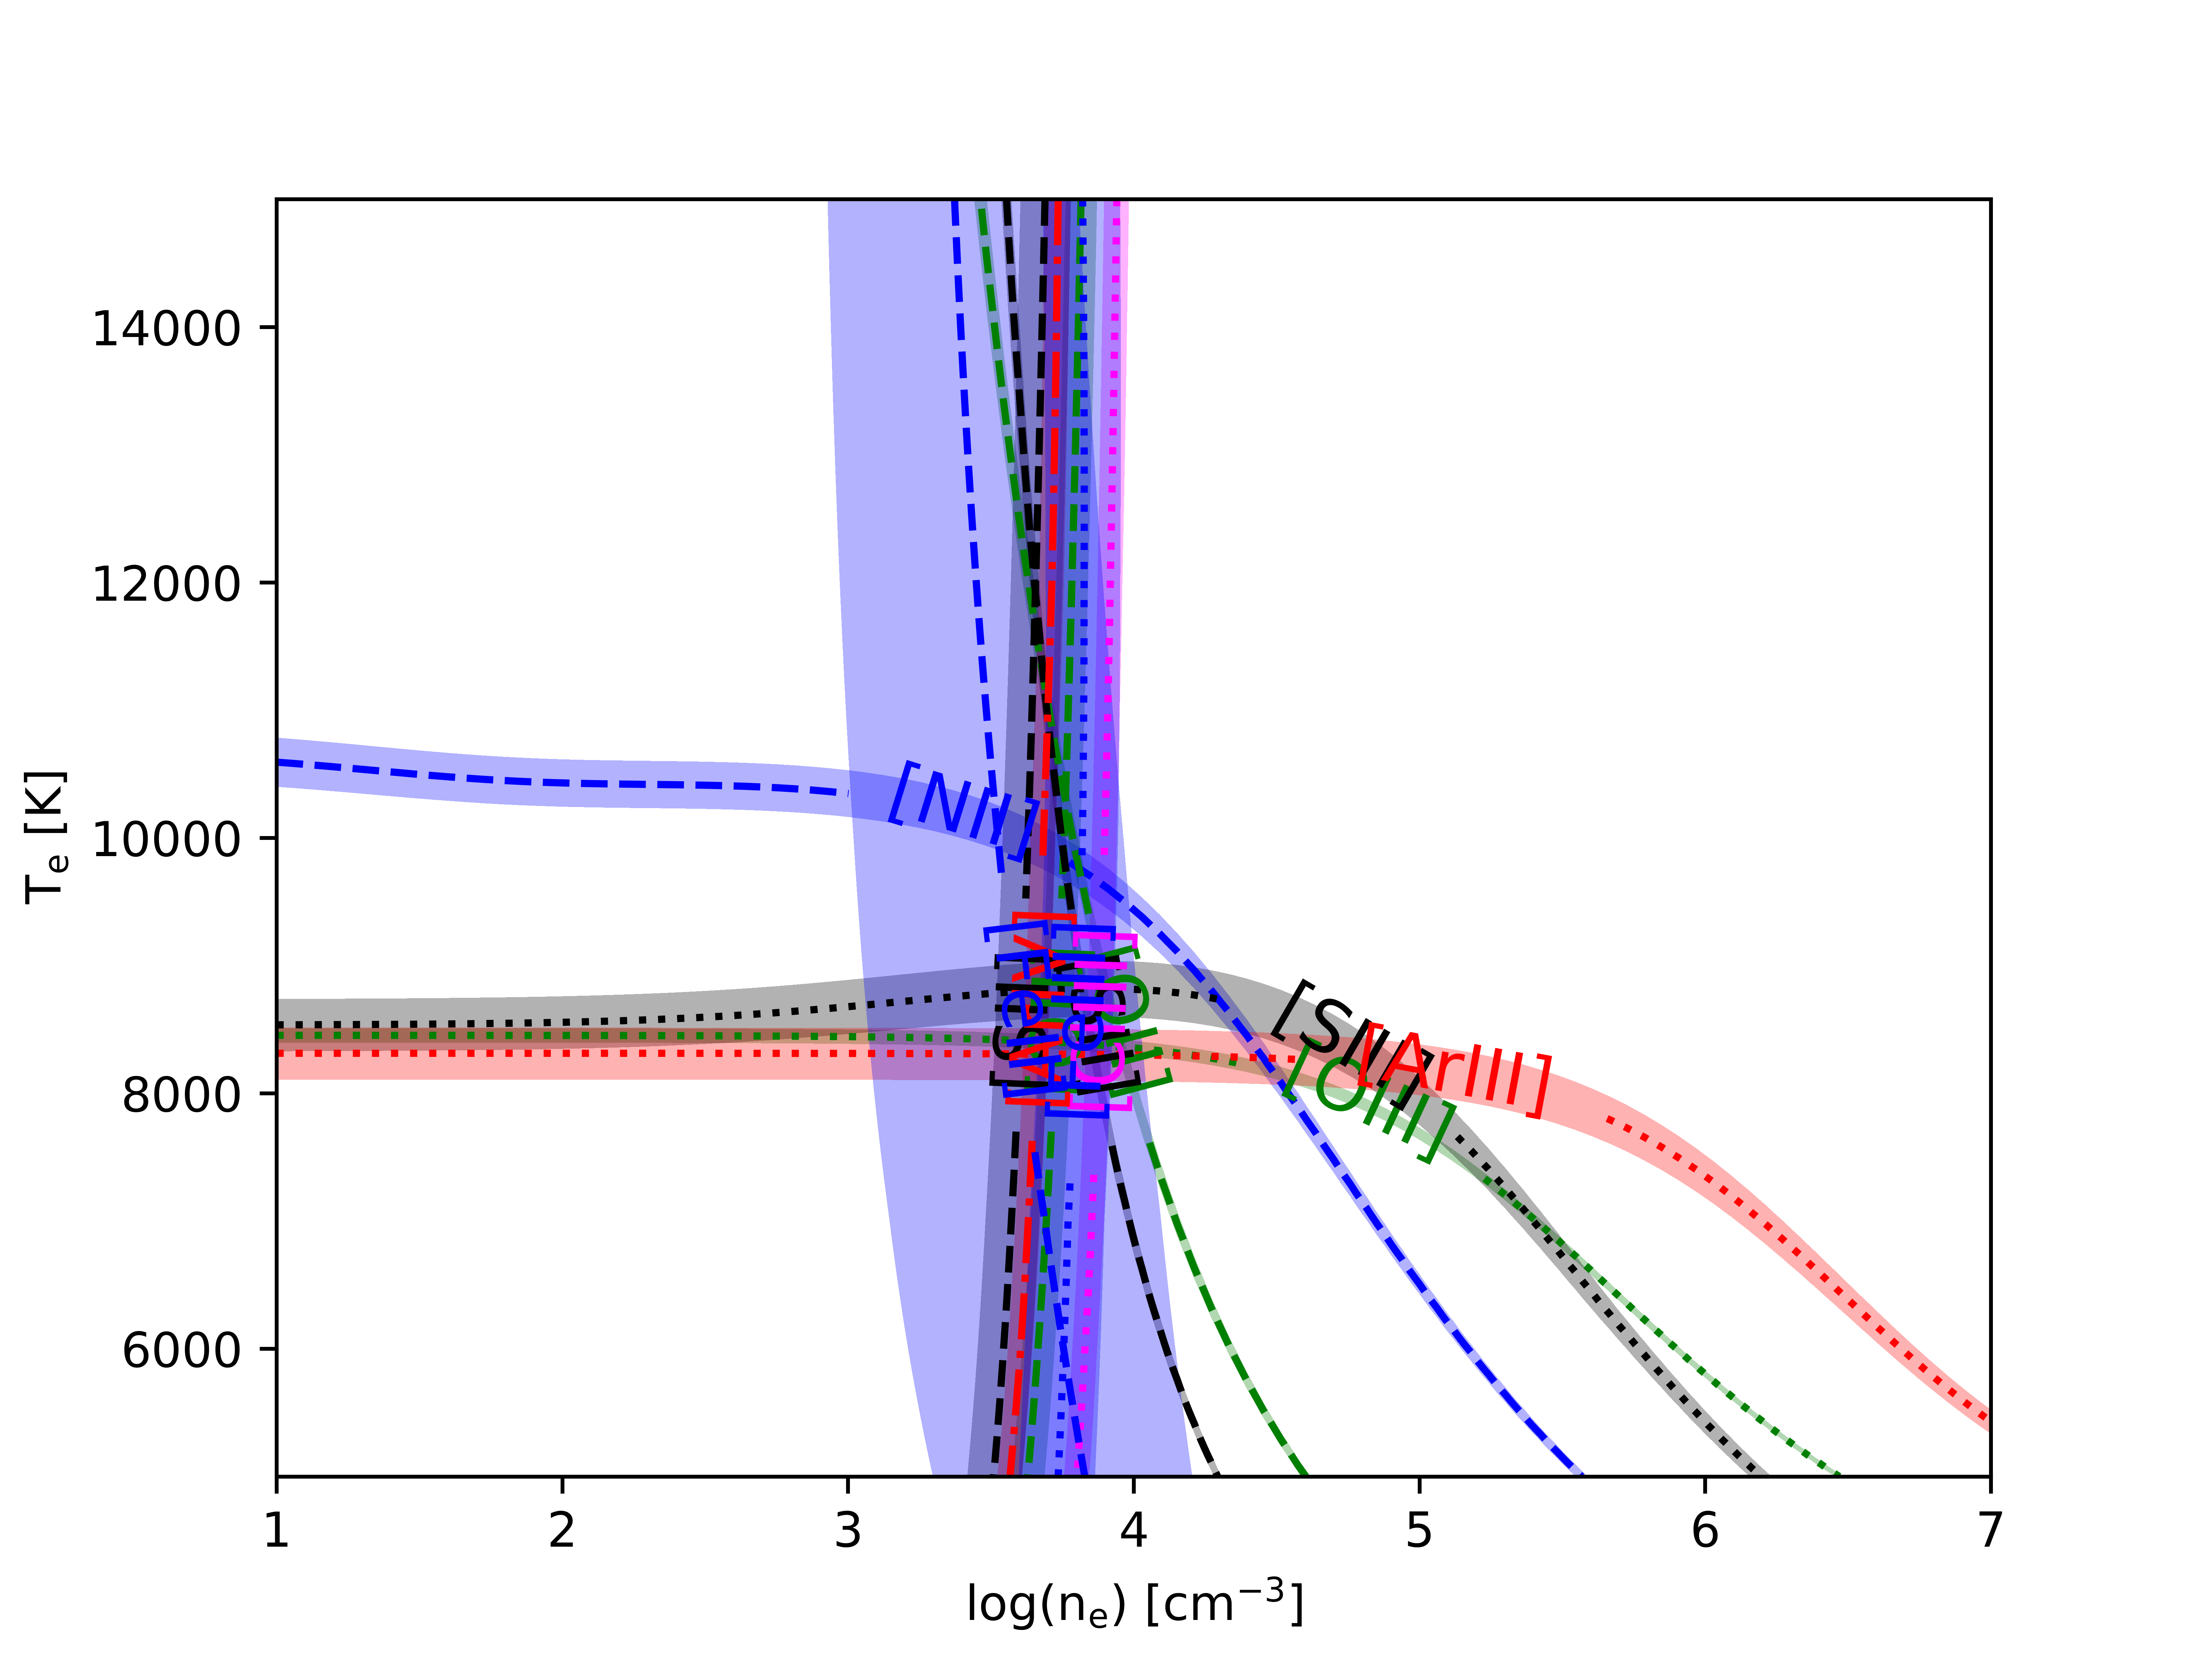
\includegraphics[height=4cm,width=\columnwidth]{neb_cut3.png}
    \centerline{(d) Cut~3, nebular component.}
  \end{minipage}
  \caption{Plasma diagnostic plots for the individual analyzed components.}
\label{fig:plasma}
\end{figure*}

\begin{figure}
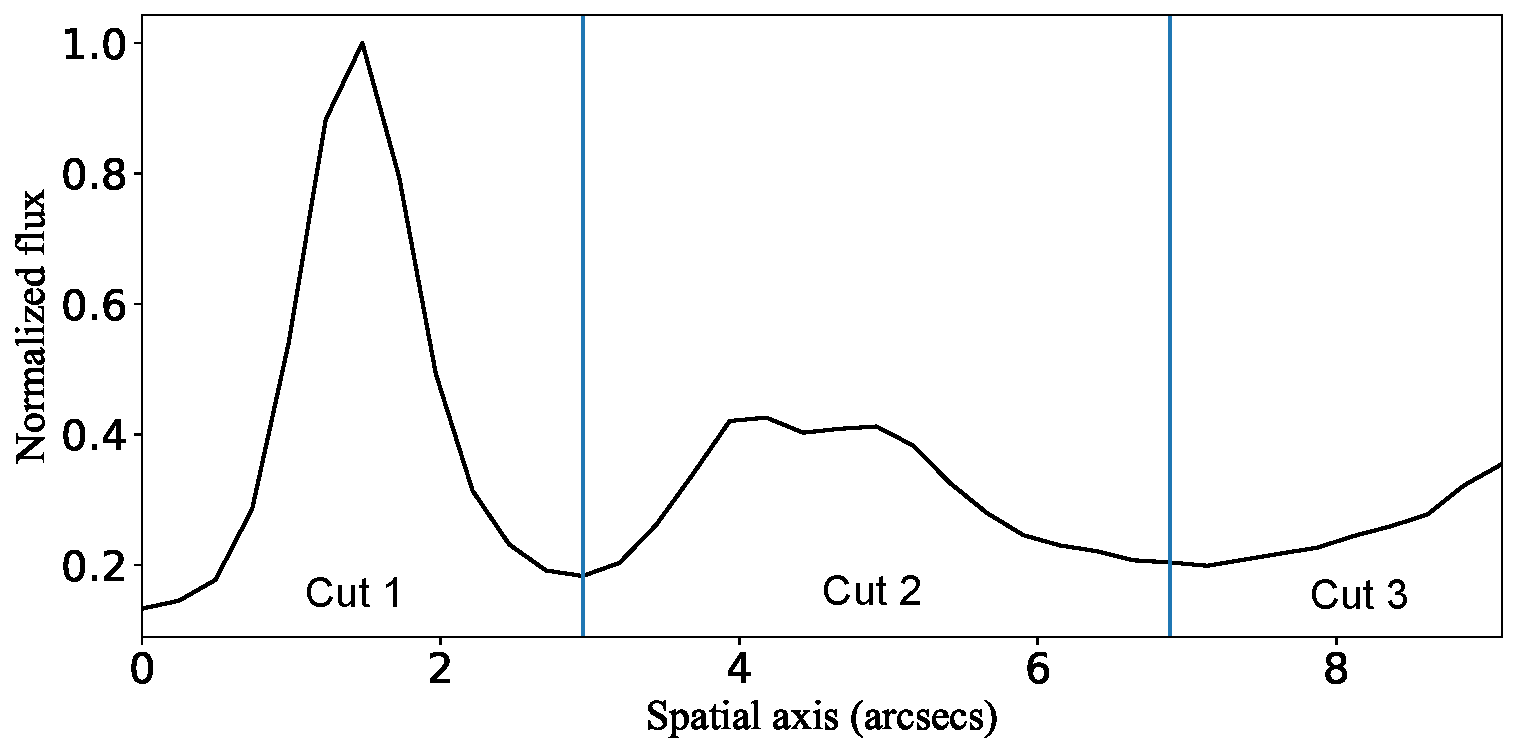
\includegraphics[width=\columnwidth]{brillo_4658_HH514.pdf}
\caption{Spatial distribution along the slit of the intensity of [Fe\thinspace III] $\lambda 4658$ line centred at a heliocentric velocity of $\sim 150 \text{ km s}^{-1}$.  The emission has been extracted from a window $\sim 45 \text{ km s}^{-1}$ wide }
\label{fig:spatial_dis}
\end{figure}


\begin{table*}
\centering
\caption{Observed [S\thinspace III] line intensity ratios with a common upper level.}
\label{tab:atomic_data_test}
%\begin{adjustbox}{width=\textwidth}
\begin{tabular}{ccccccccccccc}
\hline
Reference & 3722/6312 & 9531/9069 & 9531/8829 &9069/8829 \\
\hline

 & \multicolumn{4}{c}{{\bf Orion Nebula}}\\

\citet{Esteban04} & - & $2.39 \pm 0.51$ & $5576.37 \pm 1326.47$ & $2313.96 \pm 539.11$\\

\citet{mesadelgado09} & - & $2.32 \pm 0.19$ & - & - \\

\citet{mendez2021} Cut~1 & $0.60 \pm 0.03$ & $2.65 \pm 0.24$ & $8414.88 \pm 1221.90$ & $3204.57 \pm 455.63$\\

\citet{mendez2021} Cut~2 & - &$2.84 \pm 0.27$ & $7663.46 \pm 893.46$& $2729.17 \pm 312.05$\\

\citet{mendez2021} Cut~3 & - &$2.88 \pm 0.26$&$8259.73 \pm 1096.90$&$2875.21 \pm 365.38$\\

\citet{mendez2021} Cut~4 & - &$2.50 \pm 0.24$&$7673.32 \pm 1283.67$ & $3068.76 \pm 519.54$ \\

 
\citet{mendez2021-2} Cut~1 + NIL & - & $2.43 \pm 0.18$ &$5830.90 \pm 672.89$&$2397.19 \pm 272.37$ \\

\citet{mendez2021-2} Cut~2 & - & $2.44 \pm 0.22$ & $6752.15 \pm 1162.68$& $2789.65 \pm 474.00$ \\

\citet{mendez2021-2} NIL & - &$2.65 \pm 0.46$ &-&- \\

This work Cut~2 & $0.64 \pm 0.02$ & $2.69 \pm 0.28$ & $7771.60 \pm 1077.27$ & $2892.90 \pm 392.05$\\


This work Cut~3 & - & $2.60 \pm 0.27$ & $7388.21 \pm 972.74$ & $2828.85 \pm 372.08$\\


& \multicolumn{4}{c}{{\bf Photoionized Herbig-Haro Objects}}\\

\citet{mesadelgado09} HH~202~S & - & $2.54 \pm 0.22$ & -&-\\

\citet{mendez2021} HH~529~II &-&$2.46 \pm 0.22$&$7462.41 \pm 1822.99$&$3070.78 \pm 731.04$\\

\citet{mendez2021} HH~529~III &-&$2.45 \pm 0.29$ & - & -\\


\citet{mendez2021-2} HH~204 & - & $2.39 \pm 0.14$ & $8721.53 \pm 966.81$ & $3632.17 \pm 405.38$\\

This work HH~514~I & - & $2.60 \pm 0.32$ &-&-\\

This work HH~514~II & - & $2.55 \pm 0.38$ &-&-\\

 & \multicolumn{4}{c}{{\bf Galactic H~II regions}}\\

\citet{garciarojas04} NGC~3576 & -& - & - & $2478.77 \pm 396.99$ \\

\citet{garciarojas05} Sh~2-311& - & $2.70\pm 0.21$&-&-\\

\citet{garciarojas06} M~16 &-&$ 2.43\pm 0.29$&-&-\\

\citet{garciarojas06} M~20 & -& $ 2.29\pm 0.20$&-&-\\

\citet{garciarojas06} NGC~3603 & - & - & $5924.70 \pm 828.94$ & - \\

\citet{garciarojas07-2} M~8 &-& - &- & $2742.62 \pm 680.99$  \\

\citet{garciarojas07-2} M~17 &-& $2.51 \pm 0.25$ &-&-\\

\citet{Esteban13} NGC~2579 &- &$2.18 \pm 0.12$ &-&-\\


%---PNs---\\
%\citet{Sharpee03} IC 418 & -& 2.38 & 8798.08 & 3705.72\\

{\bf Adopted observed value} & \boldmath $0.62 \pm 0.03$ & \boldmath $2.45 \pm 0.18$& \boldmath$ 7217.60\pm 1168.83$ & \boldmath $2875.77\pm415.72$\\

 & \multicolumn{4}{c}{{\bf Theoretical Predictions}}\\

LL93-HSC95-MZ82b-KS86 &0.52& 5.52&14962.86&2710.07\\

MZ82b-HSC95-LL93  & 0.61 & 2.48 &9168.73&3697.08\\

FFTI06 &0.54& 2.47&8470.16&3430.85\\

TZS19 & 0.50 & 2.54&5504.84&2170.84\\

CHIANTI & 0.53 & 2.51&8473.87&3372.61\\

\hline
\end{tabular}
%\end{adjustbox}
\end{table*}

\begin{table*}
\centering
\caption{[S\thinspace III] $\lambda \lambda 9069, 9531$ intensity values corrected from telluric absorption bands.}
\label{tab:tellabs}
%\begin{adjustbox}{width=\textwidth}
\begin{tabular}{ccccccccccccc}
\hline
Object &   \multicolumn{2}{c}{$\lambda 9069$} & \multicolumn{2}{c}{$\lambda 9531$} & Reference\\
 & Old & New  & Old & New & \\
\hline

Orion Nebula Cut~1 & $19.713 \pm 0.985$ & $32.148\pm 1.929$& $82.845 \pm 4.971$ & $84.653 \pm 5.926$ & \multirow{4}{*}{\citet{mendez2021}}\\

Orion Nebula Cut~2 & $20.807 \pm 1.248$ &  $32.543 \pm 2.278$& $91.130\pm 5.468$&$91.438 \pm 6.401 $\\

Orion Nebula Cut~3 & $21.792\pm 1.308$ & $31.778\pm 1.907$& $91.118\pm 6.378$&$91.355 \pm 6.395$\\

Orion Nebula Cut~4 &$22.765 \pm 1.366$ & $ 34.075 \pm 2.385$ & $82.527\pm 4.952$ & $85.145\pm5.960$\\


Orion Nebula + NIL Cut~1 & $25.379\pm 1.015$ & $28.562\pm 1.428$ & $ 69.320 \pm 2.773$ & $69.330 \pm 3.466$ & \multirow{2}{*}{\citet{mendez2021-2}}\\

Orion Nebula Cut~2 & $24.746\pm 1.237$ & $30.686\pm 1.841$ & $74.642\pm 4.478$ & $74.643\pm 5.225$ \\

HH~529~II & \multicolumn{2}{c}{$40.116 \pm 2.407$} &  \multicolumn{2}{c}{$98.517 \pm 6.896$}&\multirow{2}{*}{\citet{mendez2021}}\\

HH~529~III & \multicolumn{2}{c}{$41.104 \pm 3.288$} &  \multicolumn{2}{c}{$100.396 \pm 9.036$}&\\

HH~204 & \multicolumn{2}{c}{$36.535 \pm 1.461$} & \multicolumn{2}{c}{$87.222\pm 3.489$}\\

NIL & $26.541\pm 2.919$ & $20.695\pm2.483$& $ 60.608\pm 6.667$& $55.487\pm 6.658$& \citet{mendez2021-2}\\

\hline
\end{tabular}
%\end{adjustbox}
\end{table*}




\begin{figure*}
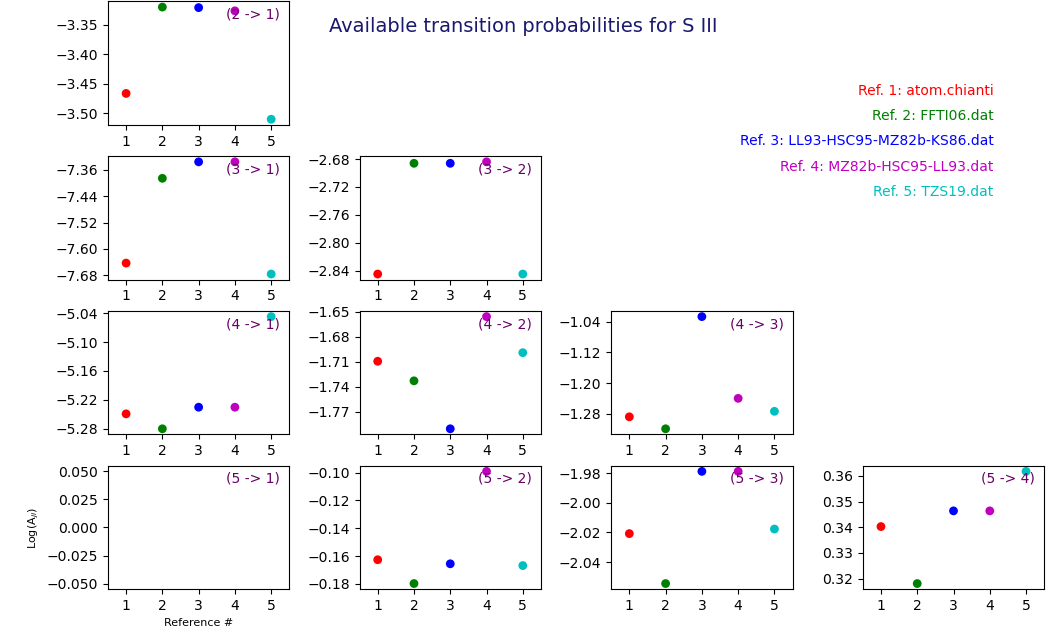
\includegraphics[width=\textwidth]{A_siii.png}
\caption{Comparison between the different values of transition probabilities of the [S\thinspace III] atom studied in this paper.}
\label{fig:A_sii}
\end{figure*}

\begin{figure*}
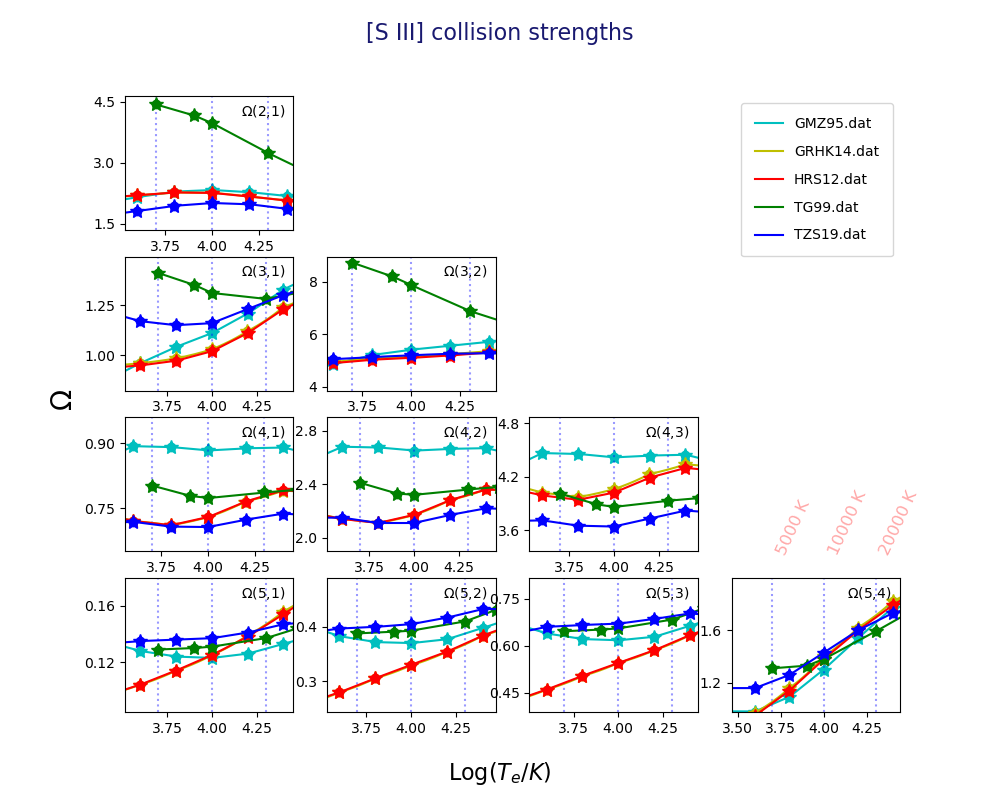
\includegraphics[width=\textwidth]{omega_siii_zoom.png}
\caption{Comparison between the different values of collision strengths of the [S\thinspace III] atom studied in this paper.}
\label{fig:omega_siii_zoom }
\end{figure*}



\begin{table*}
\centering
\caption{$T_{\rm e} \text{ ([S\thinspace III])}$ and S$^{2+}$ abundance derived with each set of collision strengths and the transition probabilities from \citet{FFTI06}. The Modified $\Omega$'s column corresponds to the GRHK14 data, with $\Omega_{9531}$, $\Omega_{9069}$ and $\Omega_{8829}$ artificially increased by 40\%.}
\label{tab:modified_data_omega}
\begin{adjustbox}{width=\textwidth}
\begin{tabular}{ccccccccccccc}
\hline
 &  GMZ95 & TG99 & HRS12 & GRHK14 & TZS19 & Modified $\Omega$'s\\
\hline

\multicolumn{7}{c}{$T_{\rm e} \text{ ([S\thinspace III])}$} \\

HH~514~I  & $8370^{+420} _{-450}$ & $7980^{+400} _{-530}$ & $8410^{+350} _{-390}$ & $8420^{+310} _{-400}$ & $7900^{+480} _{-170}$ & $8840^{+500} _{-560}$ \\

HH~514~II & $8200^{+520} _{-510}$ & $7820^{+380} _{-490}$ & $8140^{+450} _{-600}$& $8230^{+430} _{-560}$ &$7750^{+310} _{-670}$ & $8980^{+570} _{-860}$\\

Nebular Cut~2 & $8850^{+270} _{-320}$ & $8270^{+280} _{-190}$ & $8650^{+270} _{-280}$ & $8630^{+330} _{-340}$ & - & $9860^{+400} _{-470}$\\

\multicolumn{7}{c}{log(S$^{2+}$/H$^{+}$)+12} \\

HH~514~I & $7.35^{+0.07} _{-0.06}$ & $7.44^{+0.09} _{-0.07}$&$7.39 \pm 0.06 $&$7.39^{+0.07} _{-0.06}$&$7.47^{+0.08} _{-0.07}$&$7.25^{+0.08} _{-0.07}$\\

HH~514~II & $7.30^{+0.09} _{-0.07}$ & $7.39^{+0.09} _{-0.07}$& $7.36^{+0.10} _{-0.08}$&$7.35^{+0.10} _{-0.07}$& $7.43^{+0.12} _{-0.09}$ & $7.14^{+0.12} _{-0.09}$\\

Nebular Cut~2 &$6.76^{+0.05} _{-0.04}$ &$6.88^{+0.05} _{-0.04}$ &$6.86^{+0.05} _{-0.04}$ &$6.86 \pm 0.05 $ &-&$6.60^{+0.06} _{-0.05}$ \\

\hline
\end{tabular}
\end{adjustbox}
\end{table*}




\begin{table}
\caption{Fluxes and line intensities from the Proplyd 170-337 after the subtraction of the emission from the Orion Nebula.} 
%\begin{adjustbox}{width=\textwidth}
\label{tab:fluxes_proplyd}
\begin{tabular}{ccccccccc} 
\hline
$\lambda_0$ ( \AA ) & Ion & F$\left( \lambda \right)$/F$\left( \mbox{H}\beta \right)$ & I$\left( \lambda \right)$/I$\left( \mbox{H}\beta \right)$ & Err \% \\
\hline
4068.60 & $\mbox{[S}\thinspace \mbox{II]}$ & 3.423 & 4.719 & 5  \\
4076.35 & $\mbox{[S}\thinspace \mbox{II]}$ & 0.953 & 1.314 & 5  \\
4363.21 & $\mbox{[O}\thinspace \mbox{III]}$ & 2.659 & 3.308 & 4 \\
5006.84 & $\mbox{[O}\thinspace \mbox{III]}$ & 276.109 & 260.366 & 2 \\
6312.10 & $\mbox{[S}\thinspace \mbox{III]}$ & 3.652 & 2.196 & 8 &  \\
9530.60 & $\mbox{[S}\thinspace \mbox{III]}$ & 180.607 & 42.942 & 26 \\
\hline
\end{tabular}
%\end{adjustbox}
\end{table}






% Don't change these lines
\bsp	% typesetting comment
\label{lastpage}
\end{document}

% End of mnras_template.tex



datos corregidos por absorciones teluricas en este paper:

NEBULAR cut2 &$23.865\pm 1.432$& $31.843\pm2.229$ & $85.893\pm 6.013$ & $85.910 \pm  6.872$ \\ 

NEBULAR cut3 &$23.676\pm 1.420$ & $31.122\pm 2.179$ & $85.362\pm 5.122$ & $81.153\pm 5.680$\\ 


HH514I & $72.951\pm 5.836$ &$74.610\pm6.715$ & $194.920\pm 15.594$&$194.289 \pm 17.486$\\ 

HH514II & $82.483\pm 7.424$ &$87.074\pm 8.707$&$217.667\pm21.767$&$ 220.679\pm24.274 $\\ 

